\chapterimage{Pictures/chap07/checkerboard-ref-465x930.png}
\chapter{采样与重构}\label{chap:采样与重构}
\setcounter{sidenote}{1}
尽管像pbrt那样的渲染器最终输出的是彩色像素的2D网格,
但实际上入射辐射是定义在胶片平面上的连续函数。
从该连续函数计算出离散像素值的方法会显著影响渲染器生成的最终图像的质量;
如果没有仔细执行该过程,则会出现伪影\sidenote{译者注:原文artifact。}。
反之,如果执行得很好,则为此进行相对少量的额外计算就能极大提升渲染图像的质量。

本章从介绍\emph{采样理论}开始——即从定义在连续域上的函数
取出离散样本值并用它们重建与原本类似的新函数的理论。
在采样理论和低偏差点集(一种均匀分布的样本点类型)思想的基础上,
本章定义的\refvar{Sampler}{}以不同方式生成$n$维样本向量
\footnote{回想上一章中\refvar{Camera}{}用\refvar{CameraSample}{}
在胶片平面、透镜上以及时间域中取点——通过取用这些样本向量前几维来设定\refvar{CameraSample}{}值。}。
本章将介绍五种\refvar{Sampler}{}实现,涵盖了采样问题的各种方法。

本章以类\refvar{Filter}{}和\refvar{Film}{}作结。
\refvar{Filter}{}用于确定每个像素周围要融合多少倍样本量来计算最终像素值,
类\refvar{Film}{}则积累图像样本对图中像素的贡献量。

\section{采样理论}\label{sec:采样理论}
数字图像表示为一组像素值,通常对齐到矩形网格。
当在物理设备上展示数字图像时,这些值用于确定显示器上像素发射的光谱功率。
当考虑数字图像时,区分图像像素与显示器像素很重要,
前者表示一个函数在特定样本位置的值,后者是具有某个发光分布的物理对象
(例如对于LCD显示器,当以倾斜角度观察它时,颜色和亮度可能会极大变化)。
显示器用图像像素值在显示器表面构造新的图像函数。
该函数定义在显示器所有点位上,而不只是数字图像像素的无穷小点上。
这样取一组样本值并将其转换回连续函数的过程称为\keyindex{重建}{reconstruction}{}。

为了计算数字图像中的离散像素值,必须采样原始连续定义的图像函数。
在pbrt中,像大多数其他光线追踪渲染器那样,
获取图像函数有关信息的唯一方法就是通过追踪光线来对其采样。
例如,能计算胶片平面上两点间的图像函数变化边界的通用方法是不存在的。
尽管可以通过在像素位置上精确采样该函数来生成图像,
但通过在不同位置上取用更多样本并将这些关于图像函数的
额外信息融合到最终的像素值中能得到更好的结果。
实际上,为了有最佳质量的结果,计算像素值时应使得
在显示设备上重建的图像尽可能与虚拟相机胶片平面上的场景原始图像逼近。
注意这和希望显示器像素在其位置上取用图像函数实际值的目标有些微妙区别。
处理这一区别是本章实现的算法的主要目标
\footnote{本书中我们将忽略物理显示器像素特性相关问题并
    在显示器执行本节后面所述理想重建过程的假设下处理。
    该假设显然与真实显示器的工作方式不符,但这里它避免了不必要的复杂分析。
    \citet{GLASSNER1995}的第3章很好地处理了非理想显示设备
    及其对图像采样和重建过程的影响。}。

因为采样和重建过程涉及估值,所以它引入了称作\keyindex{混叠}{aliasing}{}的误差,
并会以许多方式表现出来,包括锯齿状边缘或动画中的闪烁。
产生这些误差的原因是采样过程不能捕获来自连续定义的图像函数的全部信息。

作为这些思想的一个例子,考虑一个1D函数(我们也会称之为信号)即$f(x)$,
我们可以求函数定义域中任意期望位置$x'$处的值$f(x')$。
每个这样的$x'$称为\keyindex{样本位置}{sample position}{},
$f(x')$的值称为\keyindex{样本值}{sample value}{}。
\reffig{7.1}展示了光滑1D函数的样本集,以及逼近原始函数$f$的重建信号$\tilde{f}$。
本例中,$\tilde{f}$是分段线性函数,通过线性插值相邻样本值来逼近$f$
(已经熟悉采样理论的读者会认出这是用帽函数\sidenote{译者注:原文hat function。}重建的)。
因为关于$f$唯一可用的信息是来自在位置$x'$处的采样值,
且没有关于$f$在样本间特性的信息,所以$\tilde{f}$不能完全匹配$f$。
\begin{figure}[htbp]
    \centering
    \subfloat[]{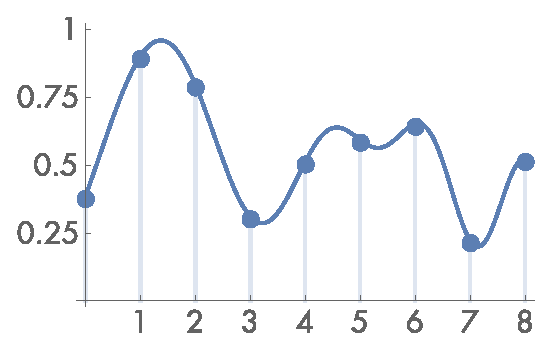
\includegraphics[width=0.4\linewidth]{chap07/point-sampling.eps}}\,\,
    \subfloat[]{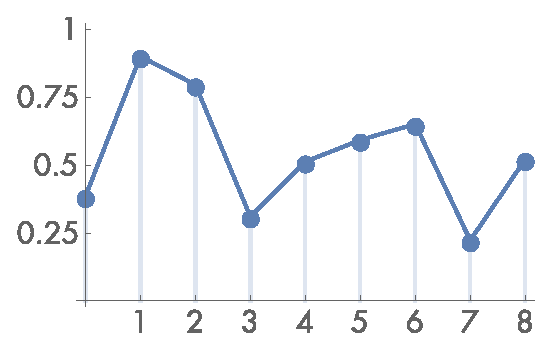
\includegraphics[width=0.4\linewidth]{chap07/linear-reconstruction.eps}}
    \caption{(a)通过取$f(x)$的\emph{样本点}集(标实心记),我们确定了函数在这些位置处的值。
        (b)样本值可用于\emph{重建}逼近$f(x)$的函数$\tilde{f}(x)$。
        \refsub{混叠}介绍的采样原理准确描述了关于$f(x)$的条件、
        所需样本的数目,以及使得$\tilde{f}(x)$和$f(x)$一模一样的重建技术。
        原始函数有时能只从样本点中完全重建的事实令人瞩目。}
    \label{fig:7.1}
\end{figure}

\keyindex{傅里叶分析}{Fourier analysis}{}可用于评估重建函数与原始函数间的匹配质量。
本节将用丰富细节来介绍一部分采样和重建过程中涉及的傅里叶分析主要思想,
但略去了许多性质的证明并跳过了与pbrt所用的采样算法没有直接关系的细节。
本章“扩展阅读”一节有关于这些话题详细信息的指引。

\subsection{频域与傅里叶变换}\label{sub:频域与傅里叶变换}
傅里叶分析的基础之一是\keyindex{傅里叶变换}{Fourier transform}{transform变换},
它在\keyindex{频域}{frequency domain}{}中来表示函数(我们称
通常的函数是在\keyindex{空域}{spatial domain}{}中表示的)。
考虑\reffig{7.2}中的两个函数。\reffig{7.2.1}中$x$的函数变化得相对较慢,
而\reffig{7.2.2}中的函数变化得迅速得多。称变化越慢的函数有越低频的分量。
\begin{figure}[htbp]
    \centering
    \subfloat[]{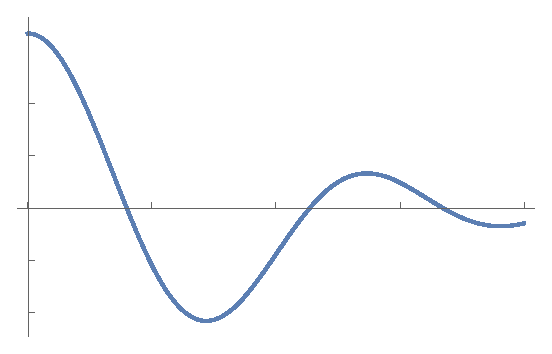
\includegraphics[width=0.32\linewidth]{chap07/func-lowfreq.eps}\label{fig:7.2.1}}\,\,\,\,
    \subfloat[]{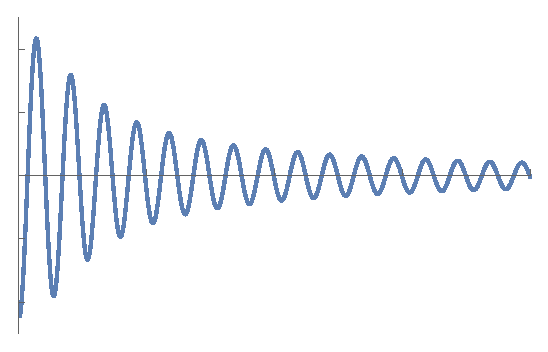
\includegraphics[width=0.32\linewidth]{chap07/func-highfreq.eps}\label{fig:7.2.2}}
    \caption{(a)低频函数和(b)高频函数。粗略地说,函数频率越高,在给定区域内变化得越快。}
    \label{fig:7.2}
\end{figure}

\reffig{7.3}展示了这两个函数在频率空间的表示;低频函数的表示比高频函数更快变为0。
\begin{figure}[htbp]
    \centering
    \subfloat[]{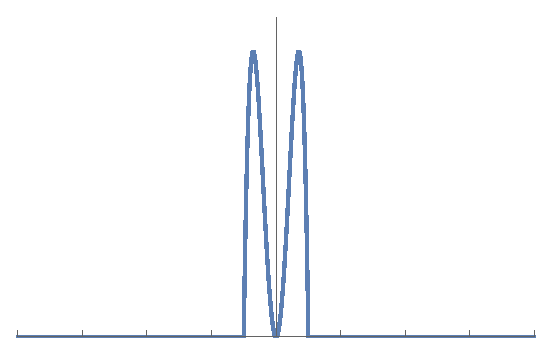
\includegraphics[width=0.32\linewidth]{chap07/fourier-lowfreq.eps}}\,\,\,\,
    \subfloat[]{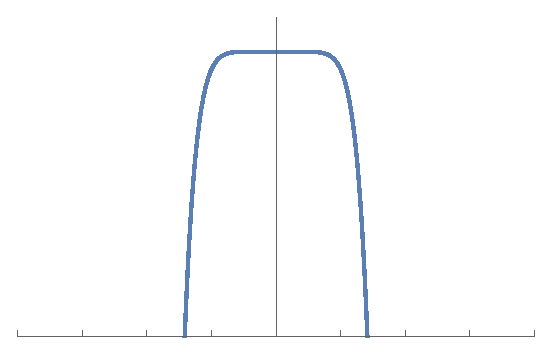
\includegraphics[width=0.32\linewidth]{chap07/fourier-highfreq.eps}}
    \caption{\reffig{7.2}中的函数的频率空间表示。本图展示了每个频率$\omega$对空域中每个函数的贡献。}
    \label{fig:7.3}
\end{figure}

许多函数可以分解为平移过的正弦曲线的加权和。
约瑟夫·傅里叶\sidenote{译者注:Jean-Baptiste Joseph Fourier,18至19世纪法国著名数学家和物理学家。}
首先描述了这一奇特事实,傅里叶变换即将函数转换为该表示。
函数的频率空间表示便于深入了解其一些特点——正弦函数的频率分布对应于原函数的频率分布。
使用该形式后,就能用傅里叶分析深入了解采样和重建过程引入的误差以及如何降低该误差带来的感知影响。

1D函数$f(x)$的傅里叶变换为\footnote{要告知读者的是,
    在不同领域中该积分前的常数并不总是一样的。例如一些作者(包括许多物理界的)
    更喜欢在两个积分前乘上$\frac{1}{\sqrt{2\pi}}$。}
\begin{align}\label{eq:7.1}
    F(\omega)=\int_{-\infty}^{\infty}f(x)\mathrm{e}^{-\mathrm{i}2\pi\omega x}\mathrm{d}x\, .
\end{align}
(回想$\mathrm{e}^{-\mathrm{i}x}=\cos x+\mathrm{i}\sin x$,其中$\mathrm{i}=\sqrt{-1}$。)
为了简便,这里我们将只考虑\keyindex{偶函数}{even function}{},
即$f(-x)=f(x)$,这种情况下$f$的傅里叶变换没有虚数项。
新函数$F$是\keyindex{频率}{frequency}{}$\omega$的函数
\footnote{本章中,我们将用符号$\omega$表示频率。在本书剩下部分中,$\omega$表示规范化的方向向量。
    这种记号的重复在使用它们的给定上下文中不应混淆。简单来说,当我们说函数的“频谱”(spectrum)时,
    我们是在说它在其频率空间表示中的频率分布,而不是和颜色相关的东西。}。
我们将用$\mathcal{F}$表示傅里叶变换运算
\sidenote{译者注:原文使用的符号是$\mathrm{F}$,这里译者换用更常用的花体$\mathcal{F}$,
    也更利于阅读时与其他符号区分。},即$\mathcal{F}\{f(x)\}=F(\omega)$。
$\mathcal{F}$显然是线性运算——即对任意标量$a$都有$\mathcal{F}\{af(x)\}=a\mathcal{F}\{f(x)\}$,
且$\mathcal{F}\{f(x)+g(x)\}=\mathcal{F}\{f(x)\}+\mathcal{F}\{g(x)\}$。

\refeq{7.1}称为\keyindex{傅里叶分析}{Fourier analysis}{}方程,有时简称\keyindex{傅里叶变换}{Fourier transform}{transform变换}。
我们也可用\keyindex{傅里叶合成}{Fourier synthesis}{}方程从频域变换回空域,
也称作\keyindex{傅里叶逆变换}{inverse Fourier transform}{transform变换}
\sidenote{译者注:大多数文献采用的傅里叶变换或逆变换定义中$\omega$是角频率,但本书的定义中$\omega$是频率。}:
\begin{align}\label{eq:7.2}
    f(x)=\int_{-\infty}^{\infty}F(\omega)\mathrm{e}^{\mathrm{i}2\pi\omega x}\mathrm{d}\omega\, .
\end{align}

\reftab{7.1}展示了许多重要函数及其频率空间表示
\sidenote{译者注:表中原文将频域函数写作$f(\omega)$,译者改为了$F(\omega)$。
    此外,表中原文对余弦函数和Shah函数的频域表示混用了系数不同的傅里叶变换定义,
    导致与本书所采用的定义不符,译者已根据本书定义对其作了修正。
    具体推导过程可参考译者补充的\refsec{译者补充:信号处理}。}。
这些函数中许多都基于狄拉克$\delta$分布
\sidenote{译者注:也称作单位\keyindex{冲激函数}{impulse function}{}、脉冲函数。},
该空间函数的定义使得$\displaystyle\int\delta(x)\mathrm{d}x=1$,且对任意$x\neq0$,都有$\delta(x)=0$。
这些性质的一个重要结论是
\begin{align*}
    \int f(x)\delta(x)\mathrm{d}x=f(0)\, .
\end{align*}

$\delta$分布不能表示为标准数学函数\sidenote{译者注:也就是说冲激函数是一种奇异函数。},
但通常可以视作以原点为中心且宽度逼近0的单位面积矩形函数\sidenote{译者注:原文box function。}的极限。
\begin{table}[htbp]
    \centering\begin{tabular}{l p{170pt}}
        \toprule
        {\bfseries 空域}                                                   & {\bfseries 频率空间表示}                                                                     \\
        \midrule
        矩形函数:$f(x)=\left\{\begin{array}{ll}
                1, & \text{若}|x|<\frac{1}{2}, \\
                0, & \text{其他}.
            \end{array}\right.$           & Sinc函数:$\displaystyle F(\omega)=\mathrm{sinc}(\omega)=\frac{\sin(\pi\omega)}{\pi\omega}$  \\
        \hline
        高斯函数:$f(x)=\mathrm{e}^{-\pi x^2}$                             & 高斯函数:$F(\omega)=\mathrm{e}^{-\pi \omega^2}$                                             \\
        \hline
        常函数:$f(x)=1$                                                   & $\delta$函数:$F(\omega)=\delta(\omega)$                                                     \\
        \hline
        余弦函数:$f(x)=\cos x$                                            & 平移的$\delta$函数:
        $F(\omega)=\frac{1}{2}(\delta(1-2\pi\omega)+\delta(1+2\pi\omega))$                                                                                                \\
        \hline
        Shah函数:$\displaystyle f(x)=III_T(x)=T\sum\limits_k\delta(x-kT)$ & $\displaystyle F(\omega)=TIII_{\frac{1}{T}}(\omega)=\sum\limits_k\delta(\omega-\frac{k}{T})$ \\
        \bottomrule
    \end{tabular}
    \caption{傅里叶变换对。空域中的函数及其频率空间表示。
        因为傅里叶变换的对称性,如果左边一列被当作频率空间,
        则右边一列是这些函数的空间等价。}
    \label{tab:7.1}
\end{table}

\subsection{理想采样与重建}\label{sub:理想采样与重建}

\subsection{混叠}\label{sub:混叠}

\section{采样接口}\label{sec:采样接口}

\subsection{基本采样器接口}\label{sub:基本采样器接口}

\begin{lstlisting}
`\initcode{Sampler Declarations}{=}\initnext{SamplerDeclarations}`
class `\initvar{Sampler}{}` {
public:
    `\refcode{Sampler Interface}{}`
    `\refcode{Sampler Public Data}{}`
protected:
    `\refcode{Sampler Protected Data}{}`
private:
    `\refcode{Sampler Private Data}{}`
};
\end{lstlisting}

\section{分层采样}\label{sec:分层采样}
我们将要介绍的首个\refvar{Sampler}{}实现会把
像素区域细分为矩形区域并在每个区域内生成单个样本。
这些区域常称为\keyindex{层}{strata}{},
而该采样器称为\refvar{StratifiedSampler}{}。
分层背后的关键思想是通过把采样域细分为不重叠区域
并从每个中取单个样本,我们更不可能错失整个图像的重要特征,
因为保证了样本不会全都挨在一起。换句话说,
如果许多样本都从样本空间中的邻近点取得则对我们没有好处,
因为每个新样本不能增加许多关于图像函数特性的新信息。
从信号处理的角度看,我们在隐式定义整体采样率,
它使得层级越小,我们拥有的层数就越多,因此采样率就越高。

分层采样器通过对层中心点施加一个至多为层的一半宽高的
随机\keyindex{扰动}{jitter}{}量来将每个样本置于每层中的随机点处。
如\refsec{采样理论}讨论的,该扰动引起的非均匀性帮助把混叠转化为噪声。
采样器还提供了非扰动模式,给出层中的均匀采样;
比起用于渲染高质量图像,该模式对于比较不同采样技术才最有用。

直接对高维采样应用分层法很快导致样本量巨大。
例如,如果我们在每个维度上把5D的图像、透镜和时间样本空间划分为四层,
则每个像素的样本总量将是$4^5=1024$.
我们可以通过在某些维度取更少的样本(或者不分层某些维度,实际上使用单层)来降低该影响,
但我们将会失去在这些维度拥有分层良好的样本的好处。
该分层问题称为\keyindex{维度灾难}{curse of dimensionality}{}。

通过为域的维度子集计算低维分层模式然后随机联合每个维度集合中的样本,
我们可以获取分层的大多数好处而不用为过多采样总量付出代价
(该过程有时称为\keyindex{填充}{padding}{})。
\reffig{7.16}展示了基本思想:我们可能只想每个像素取四个样本,
但仍得在所有维度上对样本分层。我们独立生成四个2D分层图像样本,
四个1D分层时间样本,以及四个2D分层透镜样本。
然后我们随机地为每个图像样本联合一个时间以及透镜样本值。
结果是每个像素拥有合起来良好覆盖样本空间的样本。
\begin{figure}[htbp]
    \centering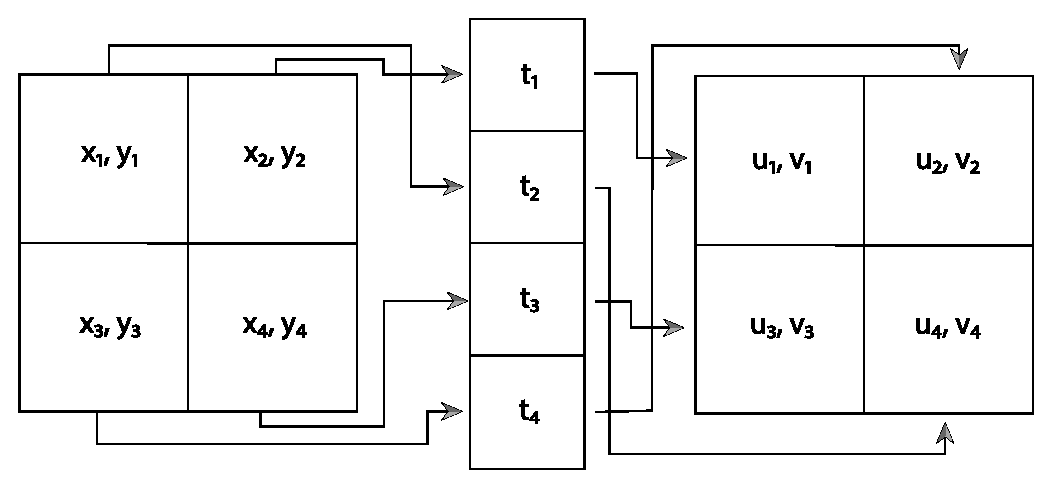
\includegraphics[width=0.8\linewidth]{chap07/Samplepadding.eps}
    \caption{我们可以生成良好的样本模式并获得分层的好处而不要求
        同时对所有采样维度分层。这里,我们已把$(x,y)$图像位置、
        时间$t$以及$(u,v)$透镜位置分为独立的层,每个都有四个区域。
        每个都是独立采样的,然后每个图像样本都随机关联一个时间样本
        和一个透镜样本。我们保留了在每个单独维度上分层的好处而不用指数级地增加样本总量。}
    \label{fig:7.16}
\end{figure}

\reffig{7.17}展示了在渲染景深时使用分层的透镜样本和
使用不分层的随机样本相比图像质量的提升。
\begin{figure}[htbp]
    \subfloat[参考]{\includegraphics[width=0.49\linewidth]{chap07/dof-ref.png}\label{fig:7.17.1}}\,
    \subfloat[随机采样]{\includegraphics[width=0.49\linewidth]{chap07/dof-random.png}\label{fig:7.17.2}}\\
    \subfloat[分层采样]{\includegraphics[width=0.49\linewidth]{chap07/dof-stratified.png}\label{fig:7.17.3}}
    \caption{渲染有景深的紫色球体时采样模式的影响。
        (a)模糊球体的高质量参考图像。(b)在每个像素中随机采样而无分层所生成的图像。
        (c)用同样数量的样本生成的图像,但用的是\refvar{StratifiedSampler}{},
        它分层了图像样本以及对该图更重要的透镜样本。对于该情形分层法做出了很大改善。}
    \label{fig:7.17}
\end{figure}

\reffig{7.18}展示比较了几种采样模式。
第一种是完全随机的模式:我们生成大量样本而完全不使用分层。
其结果很差;一些区域只有几个样本而另一些区域有好几团样本。
第二种是均匀分层模式。最后,均匀模式被扰动,
随机偏移量被加到每个样本的位置上,但仍将其保留在格子中。
这给出了比纯随机模式更好的整体分布而又保留了分层的好处,
尽管仍有一些样本团以及欠采样的区域。
\begin{figure}[htbp]
    \subfloat[]{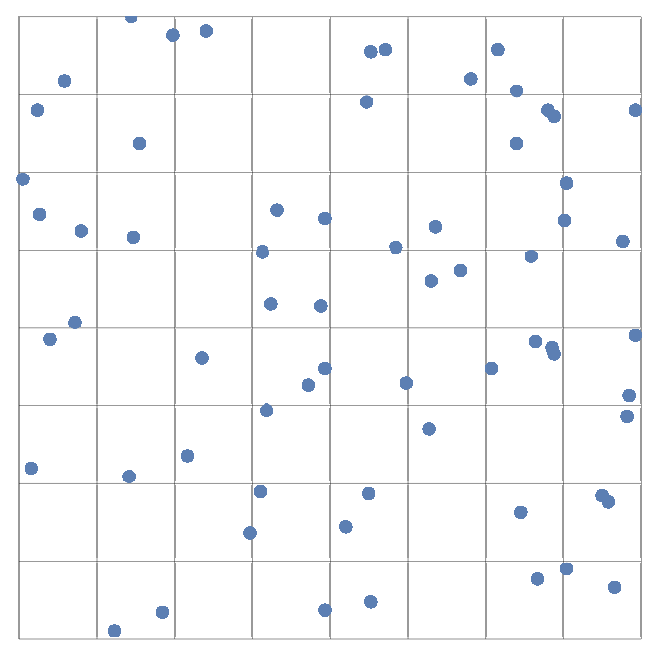
\includegraphics[width=0.49\linewidth]{chap07/random-point-samples.eps}\label{fig:7.18.1}}\,
    \subfloat[]{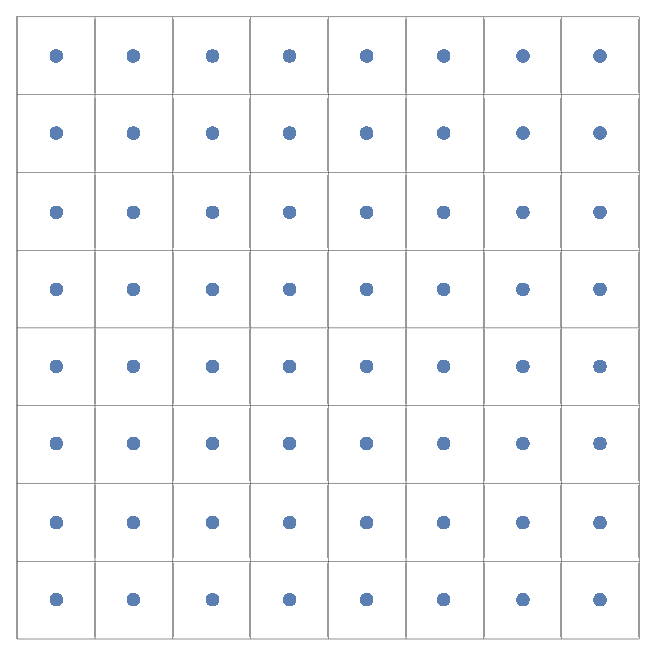
\includegraphics[width=0.49\linewidth]{chap07/uniform-point-samples.eps}\label{fig:7.18.2}}\\
    \subfloat[]{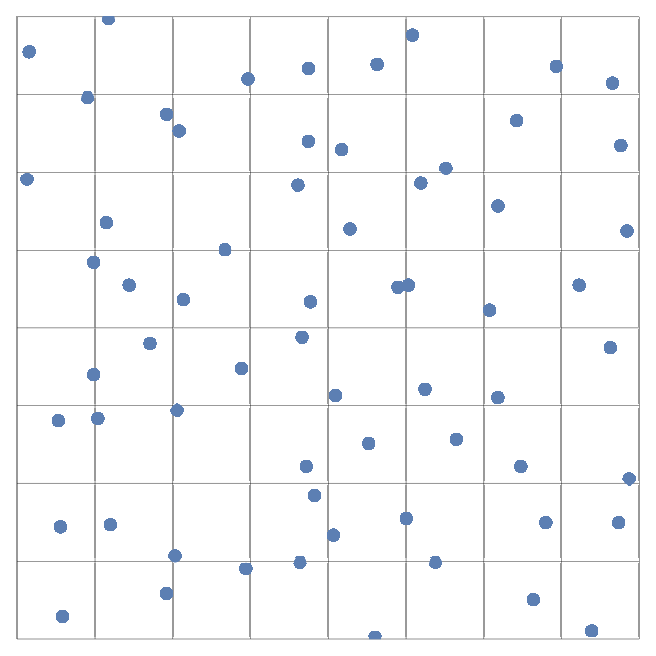
\includegraphics[width=0.49\linewidth]{chap07/jittered-point-samples.eps}\label{fig:7.18.3}}
    \caption{三种2D采样模式。(a)随机模式是无效模式,许多样本团让大片图像没有好好采样。
        (b)均匀分层模式的分布更好但会加剧混叠伪影。
        (c)分层扰动模式将来自均匀模式的混叠转化为高频噪声而仍保留了分层的好处。}
    \label{fig:7.18}
\end{figure}

\reffig{7.19}展示了用\refvar{StratifiedSampler}{}渲染的图像,
并展示了扰动的样本位置怎样将混叠伪影转化为不那么讨厌的噪声。
\begin{figure}[htbp]
    \centering
    \subfloat[参考]{\includegraphics[width=0.8\linewidth]{chap07/checkerboard-ref.png}\label{fig:7.19.1}}\\
    \subfloat[1个均匀样本]{\includegraphics[width=0.8\linewidth]{chap07/checkerboard-unif-1spp.png}\label{fig:7.19.2}}\\
    \subfloat[1个扰动样本]{\includegraphics[width=0.8\linewidth]{chap07/checkerboard-jitter-1spp.png}\label{fig:7.19.3}}\\
    \subfloat[4个扰动样本]{\includegraphics[width=0.8\linewidth]{chap07/checkerboard-jitter-4spp.png}\label{fig:7.19.4}}
    \caption{用棋盘纹理比较图像采样方法。这是幅很难渲染好的图像,
        因为当我们接近地平线时棋盘格关于像素间隔的频率趋于无穷。
        (a)参考图像,每个像素用256个样本渲染,展示了接近理想结果的样子。
        (b)每个像素只用一个样本渲染的图像,没有扰动。注意前景中格子边缘的锯齿伪影。
        还注意棋盘格函数在样本之间经历了许多周期的距离处的伪影;
        如之前介绍过的信号处理理论所料,细节错误地重复表现为低频混叠。
        (c)扰动图像样本的结果,每个像素还是只有一个样本。
        第二幅图像规则的混叠已经被替换为不那么讨厌的噪声伪影。
        (d)每个像素用四个扰动样本的结果仍然不如参考图像,但明显优于之前的结果。}
    \label{fig:7.19}
\end{figure}

\begin{lstlisting}
`\initcode{StratifiedSampler Declarations}{=}`
class `\initvar{StratifiedSampler}{}` : public `\refvar{PixelSampler}{}` {
public:
    `\refcode{StratifiedSampler Public Methods}{}`
private:
    `\refcode{StratifiedSampler Private Data}{}`
};
\end{lstlisting}
\begin{lstlisting}
`\initcode{StratifiedSampler Public Methods}{=}`
`\refvar{StratifiedSampler}{}`(int xPixelSamples, int yPixelSamples,
        bool jitterSamples, int nSampledDimensions)
    : `\refvar{PixelSampler}{}`(xPixelSamples * yPixelSamples, nSampledDimensions),
      `\refvar{xPixelSamples}{}`(xPixelSamples), `\refvar{yPixelSamples}{}`(yPixelSamples),
      `\refvar{jitterSamples}{}`(jitterSamples) { }
\end{lstlisting}
\begin{lstlisting}
`\initcode{StratifiedSampler Private Data}{=}`
const int `\initvar{xPixelSamples}{}`, `\initvar{yPixelSamples}{}`;
const bool `\initvar{jitterSamples}{}`;
\end{lstlisting}

作为\refvar{PixelSampler}{}的子类,
\refvar[StratifiedSampler::StartPixel]{StartPixel}{()}的实现必须按照传给\refvar{PixelSampler}{}
构造函数的维数{\ttfamily nSampledDimensions}一起生成1D和2D样本以及请求的数组样本。
\begin{lstlisting}
`\initcode{StratifiedSampler Method Definitions}{=}`
void `\refvar{StratifiedSampler}{}`::`\initvar[StratifiedSampler::StartPixel]{StartPixel}{}`(const `\refvar{Point2i}{}` &p) {
    `\refcode{Generate single stratified samples for the pixel}{}`
    `\refcode{Generate arrays of stratified samples for the pixel}{}`
    `\refvar{PixelSampler}{}`::StartPixel(p);
}
\end{lstlisting}

生成初始的分层样本后,它们被随机打乱;这是本节开头描述的填充方法。
如果没有进行打乱,则样本维度的值可能以某种方式相关而引发图像中的错误——
例如,用于选择胶片位置的首个2D样本和首个2D透镜样本会总是都在相邻于原点的左下方那层。
\begin{lstlisting}
`\initcode{Generate single stratified samples for the pixel}{=}`
for (size_t i = 0; i < `\refvar{samples1D}{}`.size(); ++i) {
    `\refvar{StratifiedSample1D}{}`(&`\refvar{samples1D}{}`[i][0], `\refvar{xPixelSamples}{}` * `\refvar{yPixelSamples}{}`,
                       `\refvar[PixelSampler::rng]{rng}{}`, `\refvar{jitterSamples}{}`);
    `\refvar{Shuffle}{}`(&`\refvar{samples1D}{}`[i][0], `\refvar{xPixelSamples}{}` * `\refvar{yPixelSamples}{}`, 1, `\refvar[PixelSampler::rng]{rng}{}`);
}
for (size_t i = 0; i < `\refvar{samples2D}{}`.size(); ++i) {
    `\refvar{StratifiedSample2D}{}`(&`\refvar{samples2D}{}`[i][0], `\refvar{xPixelSamples}{}`, `\refvar{yPixelSamples}{}`,
                       `\refvar[PixelSampler::rng]{rng}{}`, `\refvar{jitterSamples}{}`);
    `\refvar{Shuffle}{}`(&`\refvar{samples2D}{}`[i][0], `\refvar{xPixelSamples}{}` * `\refvar{yPixelSamples}{}`, 1, `\refvar[PixelSampler::rng]{rng}{}`);
}
\end{lstlisting}

1D和2D分层采样例程实现为实用函数。
两个都在域中给定层数上循环并在每个里面放置一个样本点。
\begin{lstlisting}
`\initcode{Sampling Function Definitions}{=}\initnext{SamplingFunctionDefinitions}`
void `\initvar{StratifiedSample1D}{}`(`\refvar{Float}{}` *samp, int nSamples, `\refvar{RNG}{}` &rng,
        bool jitter) {
    `\refvar{Float}{}` invNSamples = (`\refvar{Float}{}`)1 / nSamples;
    for (int i = 0; i < nSamples; ++i) {
        `\refvar{Float}{}` delta = jitter ? rng.`\refvar{UniformFloat}{}`() : 0.5f;
        samp[i] = std::min((i + delta) * invNSamples, `\refvar{OneMinusEpsilon}{}`);
    }
}
\end{lstlisting}

\refvar{StratifiedSample2D}{()}同样生成范围$[0,1)^2$中的样本。
\begin{lstlisting}
`\refcode{Sampling Function Definitions}{+=}\lastnext{SamplingFunctionDefinitions}`
void `\initvar{StratifiedSample2D}{}`(`\refvar{Point2f}{}` *samp, int nx, int ny, `\refvar{RNG}{}` &rng,
        bool jitter) {
    `\refvar{Float}{}` dx = (`\refvar{Float}{}`)1 / nx, dy = (`\refvar{Float}{}`)1 / ny;
    for (int y = 0; y < ny; ++y)
        for (int x = 0; x < nx; ++x) {
            `\refvar{Float}{}` jx = jitter ? rng.`\refvar{UniformFloat}{}`() : 0.5f;
            `\refvar{Float}{}` jy = jitter ? rng.`\refvar{UniformFloat}{}`() : 0.5f;
            samp->x = std::min((x + jx) * dx, `\refvar{OneMinusEpsilon}{}`);
            samp->y = std::min((y + jy) * dy, `\refvar{OneMinusEpsilon}{}`);
            ++samp;
        }
}
\end{lstlisting}

函数\refvar{Shuffle}{()}随机重排含有{\ttfamily count}个样本值的数组,
每个都有{\ttfamily nDimensions}维(换句话说,
尺寸为{\ttfamily nDimensions}的值构成的块被重排)。
\begin{lstlisting}
`\initcode{Sampling Inline Functions}{=}\initnext{SamplingInlineFunctions}`
template <typename T>
void `\initvar{Shuffle}{}`(T *samp, int count, int nDimensions, `\refvar{RNG}{}` &rng) {
    for (int i = 0; i < count; ++i) {
        int other = i + rng.`\refvar{UniformUInt32}{}`(count - i);
        for (int j = 0; j < nDimensions; ++j)
            std::swap(samp[nDimensions * i + j],
                      samp[nDimensions * other + j]);
    }
}
\end{lstlisting}

样本数组给我们出了个难题:例如若一个积分器
为像素中的每个样本请求样本向量中含64个2D样本值的数组,
则采样器有两个不同的目标要达成:
\begin{enumerate}
    \item 希望数组内的样本本身在2D上分布良好(例如通过使用$8\times8$分层网格)。
          这里的分层法会为每个单独的样本向量提升算出的结果的质量。
    \item 最好保证一个图像样本的数组中的每个样本都不要和图像中相邻样本的任何样本值太相似。
          即我们更希望点相对于其邻居能分布良好,使得在单个像素周围区域上就能很好覆盖整个样本空间。
\end{enumerate}

比起尝试同时解决这里的两个问题,\refvar{StratifiedSampler}{}只解决第一个。
本章后面的其他采样器会以更加精巧的技术回顾该问题并在不同程度上同时解决它们。

第二个复杂性来自于调用者可能会为每个图像样本请求任意数量样本的事实,
所以可能不易应用分层法。(例如,我们要怎么生成七个样本的分层2D模式?)
我们只能生成一个$n\times1$或$1\times n$的分层模式,
但这只能给我们在一个维度上分层的好处但不保证其他维度有好的模式。
方法{\ttfamily StratifiedSampler::RoundSize()}可以将请求进位到
下一个平方数,但我们将换用一种称为\keyindex{拉丁超立方采样}{Latin hypercube sampling}{}(LHS)的方法,
它能生成具有相当好分布的任意数量的任意维数样本。

LHS把每个维度轴均匀划分为$n$个区域并沿对角线在$n$个区域中的
每一个内生成一个扰动的样本,如\reffig{7.20}左边所示。
然后这些样本在每个维度上被随机打乱,生成分布良好的模式。
\begin{figure}[htbp]
    \centering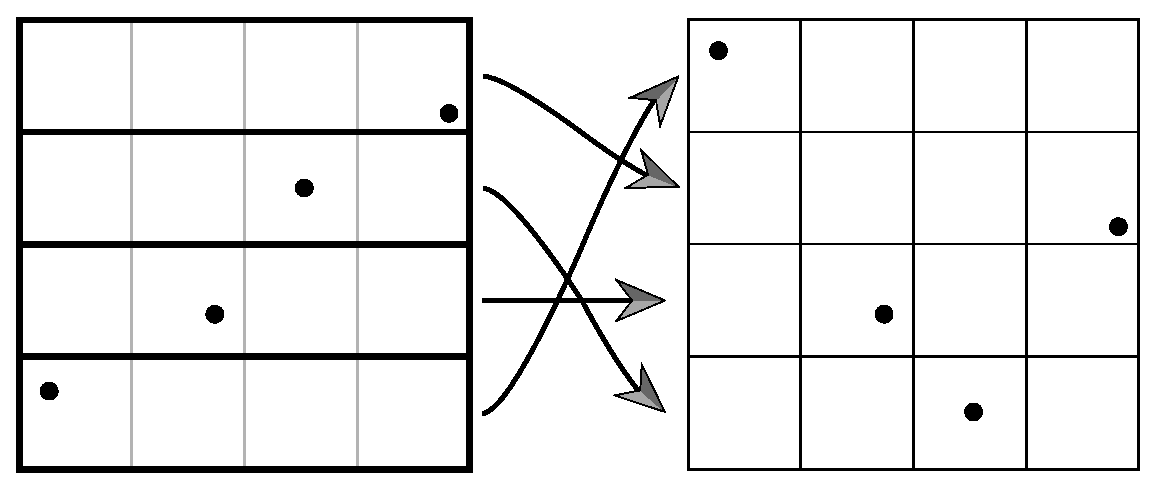
\includegraphics[width=0.8\linewidth]{chap07/LHSshuffle.eps}
    \caption{拉丁超立方采样(有时称为\protect\keyindex{$n$车采样}{$n$-rooks sampling}{})
        选择样本使得网格每行每列只出现单个样本。通过在对角线格子里生成随机样本
        然后随机重排它们的坐标可以做到这点。LHS的一个优点是它能像用分层模式那样
        生成具有良好分布的任意数量的样本,而不仅仅是$m\times n$个样本。}
    \label{fig:7.20}
\end{figure}

LHS的一个优点是当样本投影到样本维度的任意轴时它最小化了样本的聚集。
该性质与分层采样相反,后者2D模式中$n\times n$个样本里的$2n$个可能投影到每个轴上基本相同的点。
\reffig{7.21}展示了对于分层采样模式的这一最坏情况。
\begin{figure}[htbp]
    \centering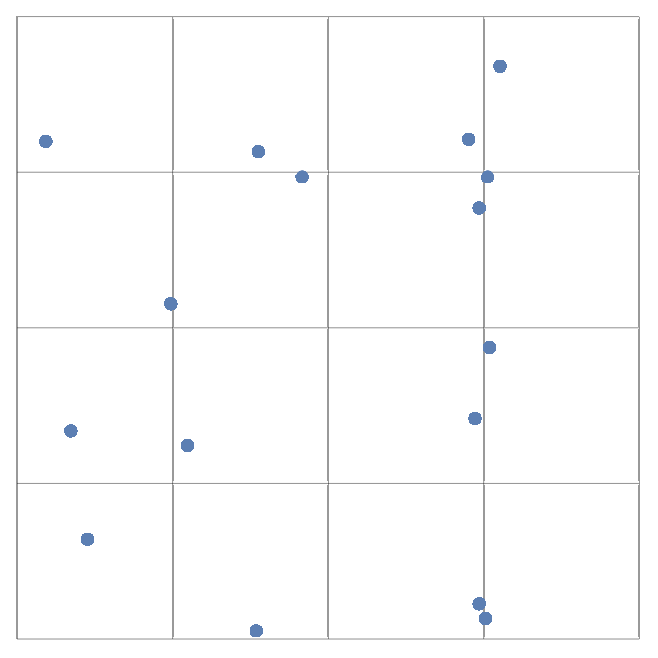
\includegraphics[width=0.4\linewidth]{chap07/stratified-bad-luck.eps}
    \caption{分层采样的一个最坏情况。在$n\times n$的2D模式中,
        多达$2n$个点可能投影到一个轴上基本相同的点。当生成像这样的“倒霉”模式时,
        用其算出的结果质量通常堪忧(这里,8个样本有几乎一样的$x$值)。}
    \label{fig:7.21}
\end{figure}

尽管解决了聚集问题,LHS对于分层采样并不是必要的改进;
很容易构造样本位置基本共线且大面积采样域没有相邻样本的情形
(例如原始样本的排列一致的时候,即让它们都保持原样)。
特别地,随着$n$增加,拉丁超立方模式比起分层模式越来越低效
\footnote{后续章节我们将回顾该问题,讨论同时是分层的且按拉丁超立方模式分布的样本模式。}。

通用的函数\refvar{LatinHypercube}{()}在任意维度生成任意数量的LHS样本。
因此数组{\ttfamily samples}中的元素数量应为{\ttfamily nSamples*nDim}。

\begin{lstlisting}
`\refcode{Sampling Function Definitions}{+=}\lastnext{SamplingFunctionDefinitions}`
void `\initvar{LatinHypercube}{}`(`\refvar{Float}{}` *samples, int nSamples, int nDim, `\refvar{RNG}{}` &rng) {
    `\refcode{Generate LHS samples along diagonal}{}`
    `\refcode{Permute LHS samples in each dimension}{}`
}
\end{lstlisting}
\begin{lstlisting}
`\initcode{Generate LHS samples along diagonal}{=}`
`\refvar{Float}{}` invNSamples = (`\refvar{Float}{}`)1 / nSamples;
for (int i = 0; i < nSamples; ++i)
    for (int j = 0; j < nDim; ++j) {
        `\refvar{Float}{}` sj = (i + (rng.`\refvar{UniformFloat}{}`())) * invNSamples;
        samples[nDim * i + j] = std::min(sj, `\refvar{OneMinusEpsilon}{}`);
    }
\end{lstlisting}

为了进行重排,该函数在样本上循环,每次在一个维度上随机重排样本点。
注意这和之前的\refvar{Shuffle}{()}例程是不一样的重排:
后者例程做一次重排,每个样本里的全部{\ttfamily nDim}个样本点是保持在一起的,
而这里是{\ttfamily nDim}次对单个维度的依次单独重排(\reffig{7.22})
\footnote{尽管不需要重排LHS模式的第一维,但这里的实现还是这样做了,
    因为让第一维的元素变为随机顺序意味着LHS模式可以与来自其他源的采样模式
    结合使用而没有其样本点间存在相关性的危险。}。
\begin{figure}[htbp]
    \centering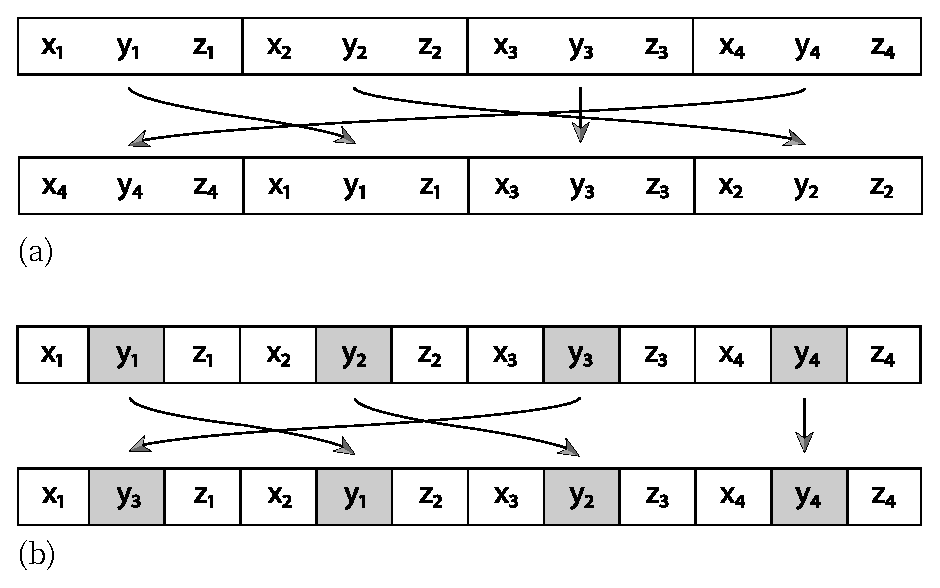
\includegraphics[width=0.8\linewidth]{chap07/Shufflepermutations.eps}
    \caption{(a)\refvar{Shuffle}{()}例程进行的重排移动附近的整块元素。
        (b)拉丁超立方采样的重排独立地排列每个维度的样本。
        这里展示了打乱四个三维元素模式的第二维样本。}
    \label{fig:7.22}
\end{figure}

\begin{lstlisting}
`\initcode{Permute LHS samples in each dimension}{=}`
for (int i = 0; i < nDim; ++i) {
    for (int j = 0; j < nSamples; ++j) {
        int other = j + rng.`\refvar{UniformUInt32}{}`(nSamples - j);
        std::swap(samples[nDim * j + i], samples[nDim * other + i]);
    }
}
\end{lstlisting}

有了函数\refvar{LatinHypercube}{()},
我们现在可以编写代码为当前像素计算样本数组了。
1D样本被分层然后随机打乱,而2D样本用拉丁超立方采样生成。
\begin{lstlisting}
`\initcode{Generate arrays of stratified samples for the pixel}{=}`
for (size_t i = 0; i < `\refvar{samples1DArraySizes}{}`.size(); ++i)
    for (int64_t j = 0; j < `\refvar{samplesPerPixel}{}`; ++j) {
        int count = `\refvar{samples1DArraySizes}{}`[i];
        `\refvar{StratifiedSample1D}{}`(&`\refvar{sampleArray1D}{}`[i][j * count], count, `\refvar[PixelSampler::rng]{rng}{}`,
                           `\refvar{jitterSamples}{}`);
        `\refvar{Shuffle}{}`(&`\refvar{sampleArray1D}{}`[i][j * count], count, 1, `\refvar[PixelSampler::rng]{rng}{}`);
    }
for (size_t i = 0; i < `\refvar{samples2DArraySizes}{}`.size(); ++i)
    for (int64_t j = 0; j < `\refvar{samplesPerPixel}{}`; ++j) {
        int count = `\refvar{samples2DArraySizes}{}`[i];
        `\refvar{LatinHypercube}{}`(&`\refvar{sampleArray2D}{}`[i][j * count].x, count, 2, `\refvar[PixelSampler::rng]{rng}{}`);
    }
\end{lstlisting}

我们将用\reffig{7.23}中的场景来阐述一些\refvar{Sampler}{}实现的性质。
\begin{figure}[htbp]
    \centering\includegraphics[width=0.75\linewidth]{chap07/area-light-example.png}
    \caption{面光源采样示例场景。}
    \label{fig:7.23}
\end{figure}

\reffig{7.24}展示了对于\refvar{DirectLightingIntegrator}{}而言来自好样本的提升。
第一幅图像每个像素用1个图像样本算得,每个有16个阴影样本。
第二幅每个像素用16个图像样本,每个有1个阴影样本。
因为\refvar{StratifiedSampler}{}能为第一种情况生成良好的LHS模式,
所以即使在取用的阴影样本总数相同时,其阴影质量也好得多。

\begin{figure}[htbp]
    \centering
    \subfloat[1个图像样本,16个阴影样本]{\includegraphics[width=\linewidth]{chap07/shadow-1-16.png}\label{fig:7.24.1}}\\
    \subfloat[16个图像样本,1个阴影样本]{\includegraphics[width=\linewidth]{chap07/shadow-16-1.png}\label{fig:7.24.2}}
    \caption{用来自分层采样器的样本采样面光源。
        (a)展示了每个像素用1个图像样本和16个阴影样本的结果,
        而(b)展示了用16个图像样本且每个只有1个阴影样本的结果。
        两种情况阴影样本的总数是一样的,但因为每个图像样本用16个阴影样本的版本
        可以使用LHS模式,像素区域内所有阴影样本都良好分布,而第二幅图像里
        这里的实现没有办法防止它们分布得很差。差别是惊人的。}
    \label{fig:7.24}
\end{figure}

\section{Halton采样器}\label{sec:Halton采样器}

\subsection{Hammersley和Halton序列}\label{sub:Hammersley和Halton序列}
\begin{lstlisting}
`\initcode{Low Discrepancy Function Definitions}{=}\initnext{LowDiscrepancyFunctionDefinitions}`
`\refvar{Float}{}` `\initvar{RadicalInverse}{}`(int baseIndex, uint64_t a) {
    switch (baseIndex) {
        case 0:
            `\refcode{Compute base-2 radical inverse}{}`
        case 1: return `\refvar{RadicalInverseSpecialized}{}`<3>(a);
        case 2: return `\refvar{RadicalInverseSpecialized}{}`<5>(a);
        case 3: return `\refvar{RadicalInverseSpecialized}{}`<7>(a);
        `\refcode{Remainder of cases for RadicalInverse()}{}`
    }
}
\end{lstlisting}

\section{(0,2)序列采样器}\label{sec:(0,2)序列采样器}
\begin{remark}
    本节含有高级内容,第一次阅读时可以跳过。
\end{remark}

另一个生成高质量样本的方法是利用某些低偏差序列的显著性质
即允许我们满足两个想要的样本性质(其中仅一个用\refvar{StratifiedSampler}{}满足了):
它们为图像样本的一个像素值生成样本向量使得每个像素样本的样本值都彼此间分布良好,
同时该像素中所有像素样本的样本值集合也整体上分布良好。

该序列使用Sobol\footnote{\protect\refsec{Sobol采样器}的\refvar{SobolSampler}{}使用了
    Sobol序列的所有维度。}推导出的低偏差序列的前两维。
该序列是一种特殊类型的低偏差序列,称为$(0,2)$序列。
$(0,2)$序列以非常常规的方式分层。例如,$(0,2)$序列中的前16个样本
满足来自\refsec{分层采样}中分层采样的分层约束,
意味着每个范围为$\displaystyle\left(\frac{1}{4},\frac{1}{4}\right)$的矩形中只存在一个样本。
然而它们还满足拉丁超立方约束,即在每个范围为$\displaystyle\left(\frac{1}{16},1\right)$和
$\displaystyle\left(1,\frac{1}{16}\right)$的矩形中只有一个样本。
此外,在每个范围为$\displaystyle\left(\frac{1}{2},\frac{1}{8}\right)$和
$\displaystyle\left(\frac{1}{8},\frac{1}{2}\right)$的矩形中只有一个样本。

\reffig{7.28}展示了划分域的所有可能,其中$(0,2)$序列前16个样本都满足分层性质。
从该模式中获取的每组含16个样本的后续序列也都满足这些分布性质。
\begin{figure}[htbp]
    \centering
    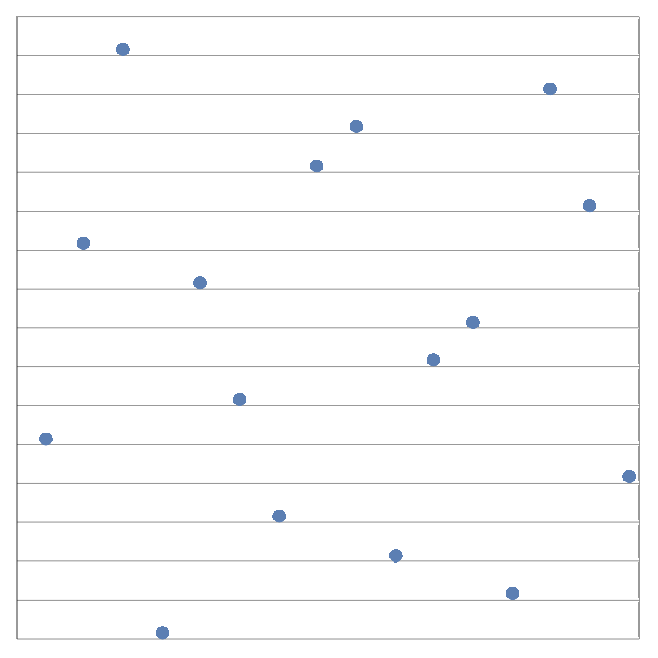
\includegraphics[width=0.49\linewidth]{chap07/elementary1x16.eps}\,
    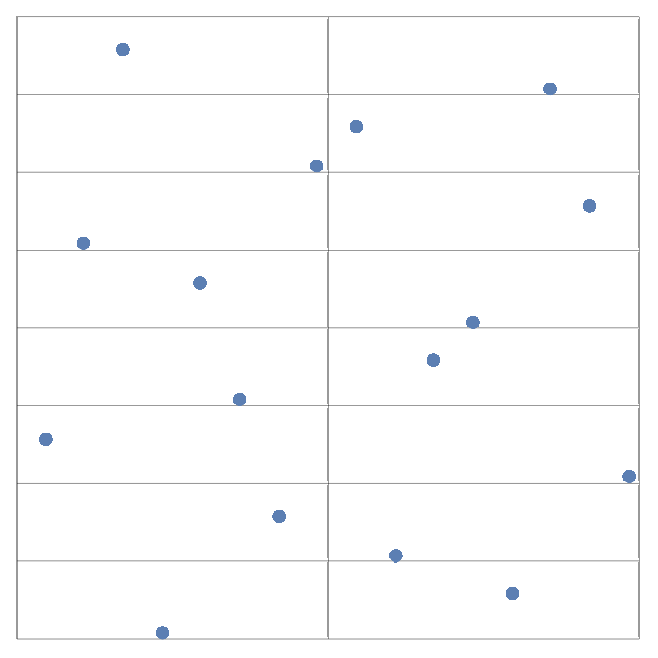
\includegraphics[width=0.49\linewidth]{chap07/elementary2x8.eps}\\
    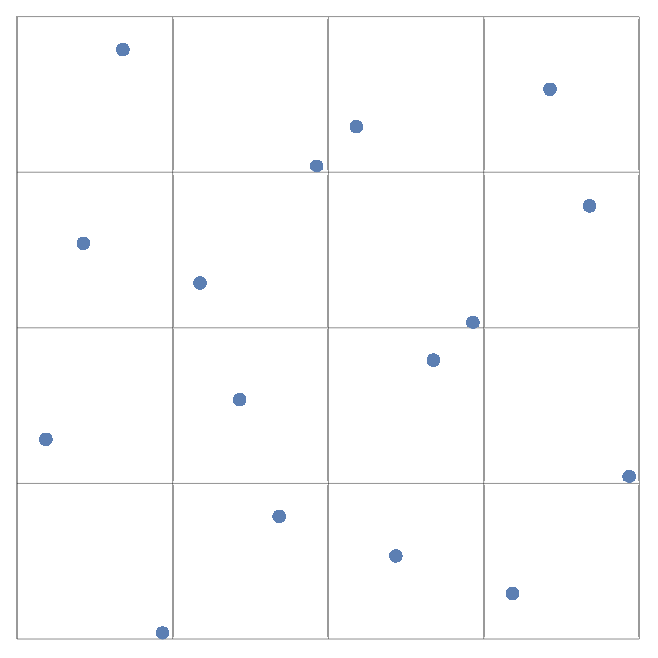
\includegraphics[width=0.49\linewidth]{chap07/elementary4x4.eps}\,
    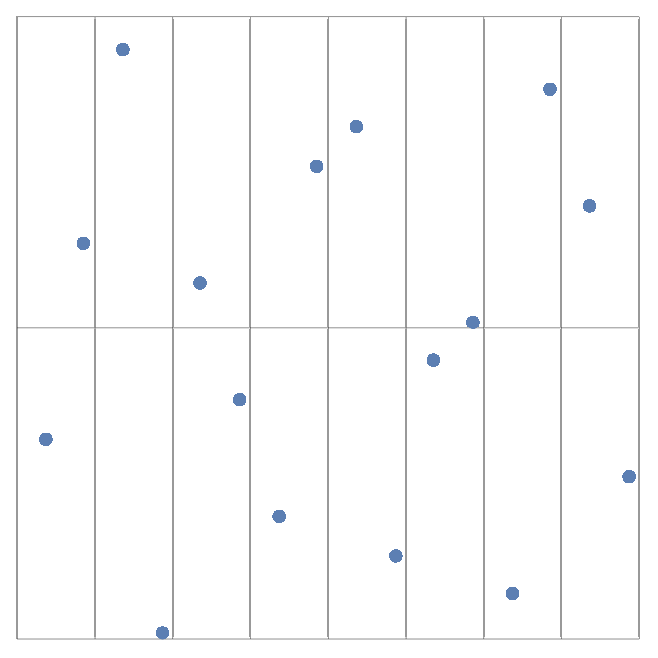
\includegraphics[width=0.49\linewidth]{chap07/elementary8x2.eps}\\
    \includegraphics[width=0.49\linewidth]{chap07/elementary16x1.eps}
    \caption{在所有以2为底数的基本区间中都只有单个样本的采样模式。
        它同时满足$4\times4$分层和拉丁超立方约束以及所示的其他两个分层约束。}
    \label{fig:7.28}
\end{figure}

通常任何来自$(0,2)$序列的长为$2^{l_1+l_2}$的序列(其中$l_i$为非负整数)
都满足该一般分层约束。以2为底的两维的\keyindex{基本区间}{elementary interval}{}定义为
\begin{align*}
    E=\left\{\left[\frac{a_1}{2^{l_1}},\frac{a_1+1}{2^{l_1}}\right)\times\left[\frac{a_2}{2^{l_2}},\frac{a_2+1}{2^{l_2}}\right)\right\}\, ,
\end{align*}
其中整数$a_i=0,1,2\ldots,2^{l_i}-1$.
该序列中前$2^{l_1+l_2}$个值中的每一个样本都在相应基本区间中。
此外,后续每$2^{l_1+l_2}$个值构成的集合也满足同样的性质。

现在为了理解怎样把$(0,2)$序列应用于生成2D样本,
考虑有$2\times2$图像样本的像素,每个含$4\times4$个2D样本构成的数组。
依据相应的基本区间集,$(0,2)$序列前$(2\times2)\times(4\times4)=2^6$个值相互之间分布良好。
此外依据其相应的基本区间,前$4\times4=2^4$个样本自己也分布良好,
其后的$2^4$个也是这样,以此类推。因此,我们可以为一个像素的
首个图像样本的$4\times4$数组样本使用前16个$(0,2)$序列样本,
然后下一个图像样本用接下来的16个,以此类推。
结果是分布非常良好的样本点集。

\subsection{用生成器矩阵采样}\label{sub:用生成器矩阵采样}
比起\refvar{HaltonSampler}{},Sobol序列基于不同的样本点生成机制,
它在各维度上使用了倒根。即使将倒根函数中的整数除法转化为乘法和位移,
高质量高分辨率渲染所需的计算数十亿样本的计算量也会很大。
大部分计算开销来自于在天生是2进制的计算机上执行不以2为底的计算
(考虑代码片\refcode{Compute base-2 radical inverse}{}和模板函数\refvar{RadicalInverseSpecialized}{()}间的差别)。


\section{最大化最小距离采样器}\label{sec:最大化最小距离采样器}


\section{Sobol采样器}\label{sec:Sobol采样器}
\begin{remark}
    本节含有高级内容,第一次阅读时可以跳过。
\end{remark}

本章最后一个\refvar{Sampler}{}基于一系列Sobol确定的生成矩阵。
来自这些矩阵生成的序列样本的区别在于能非常高效地实现——
因为是完全基于2进制计算的——而且在样本向量的全部$n$个维度上都分布得极好。
\reffig{7.34}展示了前几个Sobol生成矩阵。
\begin{figure}[htbp]
    \centering
    \includegraphics[width=0.24\linewidth]{chap07/sobol0.png}\,
    \includegraphics[width=0.24\linewidth]{chap07/sobol1.png}\,
    \includegraphics[width=0.24\linewidth]{chap07/sobol2.png}\,
    \includegraphics[width=0.24\linewidth]{chap07/sobol3.png}
    \caption{Sobol序列前四维的生成矩阵。注意其规则的结构。}
    \label{fig:7.34}
\end{figure}

\reffig{7.35}用景深测试场景比较了Sobol样本以及分层和Halton点。
\begin{figure}[htbp]
    \subfloat[分层采样]{\includegraphics[width=0.49\linewidth]{chap07/dof-stratified.png}\label{fig:7.35.1}}\,
    \subfloat[Halton采样]{\includegraphics[width=0.49\linewidth]{chap07/dof-halton.png}\label{fig:7.35.2}}\\
    \subfloat[Sobol采样]{\includegraphics[width=0.49\linewidth]{chap07/dof-sobol.png}\label{fig:7.35.3}}
    \caption{为渲染景深比较分层、Halton以及Sobol采样器。
        (a)用\refvar{StratifiedSampler}{}渲染的图像,
        (b)用\refvar{HaltonSampler}{}渲染的图像,以及
        (c)用\refvar{SobolSampler}{}渲染的图像。
        两个低偏差采样器都比分层采样器要好。尽管使用\refvar{SobolSampler}{}的该欠采样图像
        能看到结构化的网格伪影,但Sobol序列经常提供比Halton序列更快的收敛速度。}
    \label{fig:7.35}
\end{figure}

Sobol点的缺点是它们在收敛前容易出现结构化网格伪影;
在\reffig{7.36}展示的图像样本点中可以看出该问题。
\begin{figure}[htbp]
    \centering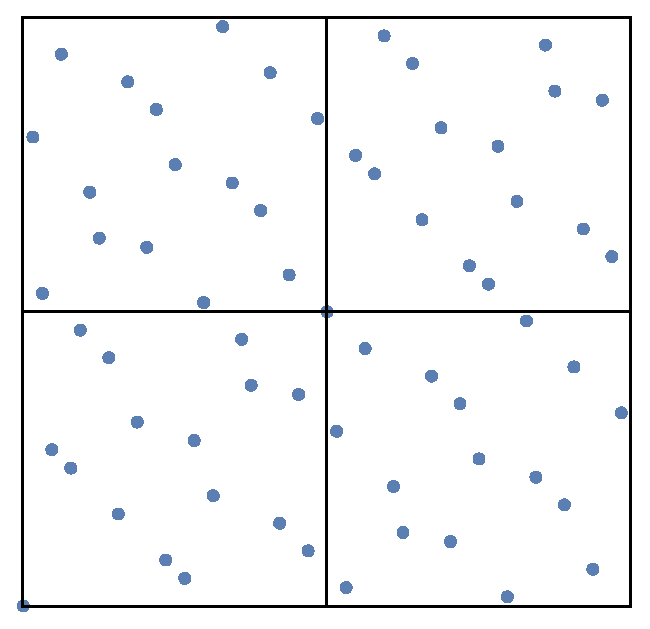
\includegraphics[width=0.5\linewidth]{chap07/sobol2x2pix.eps}
    \caption{$2\times2$像素的网格,每个用16个Sobol样本采样。
        注意有大量结构,且许多样本互相靠近。该序列在样本向量全部$n$个维度上
        极好的分布性质通常弥补了这些缺点。}
    \label{fig:7.36}
\end{figure}

在\reffig{7.37}的图像中该结构是可见的。
该缺点换来的是,Sobol序列在样本序列全部$n$个维度上分布得极其好。
\begin{figure}[htbp]
    \centering
    \subfloat[Halton采样器]{\includegraphics[width=\linewidth]{chap07/car-halton-undersampled.png}\label{fig:7.37.1}}\\
    \subfloat[Sobol采样器]{\includegraphics[width=\linewidth]{chap07/car-sobol-undersampled.png}\label{fig:7.37.2}}
    \caption{用(a)Halton采样器和(b)Sobol采样器渲染的欠采样图像。
        虽然具有不同的视觉特征,但两个都展现出可见的结构。
        特别是Sobol序列展现出清晰可见的棋盘结构。}
    \label{fig:7.37}
\end{figure}

\begin{lstlisting}
`\initcode{SobolSampler Declarations}{=}`
class `\initvar{SobolSampler}{}` : public `\refvar{GlobalSampler}{}` {
public:
    `\refcode{SobolSampler Public Methods}{}`
private:
    `\refcode{SobolSampler Private Data}{}`
};
\end{lstlisting}

\refvar{SobolSampler}{}用能让样本域$[0,1)^2$覆盖住要采样的图像区域
的最小幂2值来均匀缩放前两维。像\refvar{HaltonSampler}{}那样,
选择该特定缩放方案是为了让计算从像素坐标到每个像素内样本索引的逆映射更容易。
\begin{lstlisting}
`\initcode{SobolSampler Public Methods}{=}`
`\refvar{SobolSampler}{}`(int64_t samplesPerPixel, const `\refvar{Bounds2i}{}` &sampleBounds)
    : `\refvar{GlobalSampler}{}`(`\refvar{RoundUpPow2}{}`(samplesPerPixel)),
      `\refvar{sampleBounds}{}`(sampleBounds) {
    `\refvar{resolution}{}` = `\refvar{RoundUpPow2}{}`(std::max(sampleBounds.`\refvar{Diagonal}{}`().x,
                                      sampleBounds.`\refvar{Diagonal}{}`().y));
    `\refvar{log2Resolution}{}` = `\refvar{Log2Int}{}`(`\refvar{resolution}{}`);
}
\end{lstlisting}
\begin{lstlisting}
`\initcode{SobolSampler Private Data}{=}`
const `\refvar{Bounds2i}{}` `\initvar{sampleBounds}{}`;
int `\initvar{resolution}{}`, `\initvar{log2Resolution}{}`;
\end{lstlisting}

如果采样域$[0,1)^2$已被缩放$2^{\text{\ttfamily log2Resolution}}$倍
以覆盖像素采样区域,则函数\refvar{SobolIntervalToIndex}{()}返回
像素{\ttfamily p}内第{\ttfamily sampleNum}个样本的索引。
\begin{lstlisting}
`\refcode{Low Discrepancy Declarations}{+=}\lastcode{LowDiscrepancyDeclarations}`
inline uint64_t `\initvar{SobolIntervalToIndex}{}`(const uint32_t log2Resolution,
    uint64_t sampleNum, const `\refvar{Point2i}{}` &p);
\end{lstlisting}

用于推导它所实现的算法的一般方法和Halton采样器在其方法\linebreak
\refvar{GetIndexForSample}{()}中用的一样。
这里用幂2缩放意味着缩放值以2为底的对数给出了
构建缩放后样本整数部分的积${\bm C}[d_i(a)]^{\mathrm{T}}$的位数。
为了求得缩放后能给出特定整数值的$a$值,我们可以计算$\bm C$的逆:设
\begin{align*}
    v={\bm C}[d_i(a)]^{\mathrm{T}}\, ,
\end{align*}
则等价地
\begin{align*}
    {\bm C}^{-1}v=[d_i(a)]^{\mathrm{T}}\, .
\end{align*}
我们这里不会介绍该方法的实现。
\begin{lstlisting}
`\initcode{SobolSampler Method Definitions}{=}\initnext{SobolSamplerMethodDefinitions}`
int64_t `\refvar{SobolSampler}{}`::`\initvar[SobolSampler::GetIndexForSample]{\refvar{GetIndexForSample}{}}{}`(int64_t sampleNum) const {
    return `\refvar{SobolIntervalToIndex}{}`(`\refvar{log2Resolution}{}`, sampleNum,
        `\refvar{Point2i}{}`(`\refvar{currentPixel}{}` - `\refvar{sampleBounds}{}`.`\refvar{pMin}{}`));
}
\end{lstlisting}

\section{图像重构}\label{sec:图像重构}

\subsection{滤波器函数}\label{sub:滤波器函数}

\begin{lstlisting}
`\initcode{Filter Declarations}{=}`
class `\initvar{Filter}{}` {
public:
    `\refcode{Filter Interface}{}`
    `\refcode{Filter Public Data}{}`
};
\end{lstlisting}

{\noindent\hfil$=========$\hfil{\color{red}{施工分割线}}\hfil$=========$\
\section{胶片与成像管道}\label{sec:胶片与成像管道}

\subsection{胶片类}\label{sub:胶片类}

\begin{lstlisting}
`\initcode{Film Declarations}{=}\initnext{FilmDeclarations}`
class `\initvar{Film}{}` {
public:
    `\refcode{Film Public Methods}{}`
    `\refcode{Film Public Data}{}`
private:
    `\refcode{Film Private Data}{}`
    `\refcode{Film Private Methods}{}`
};
\end{lstlisting}

\begin{lstlisting}
`\initcode{Film Method Definitions}{=}\initnext{FilmMethodDefinitions}`
`\refvar{Film}{}`::`\refvar{Film}{}`(const `\refvar{Point2i}{}` &resolution, const `\refvar{Bounds2f}{}` &cropWindow,
        std::unique_ptr<`\refvar{Filter}{}`> filt, `\refvar{Float}{}` `\refvar{diagonal}{}`,
        const std::string &`\refvar{filename}{}`, `\refvar{Float}{}` `\refvar{scale}{}`)
    : `\refvar{fullResolution}{}`(resolution), `\refvar{diagonal}{}`(`\refvar{diagonal}{}` * .001),
    `\refvar{filter}{}`(std::move(filt)), `\refvar{filename}{}`(`\refvar{filename}{}`), `\refvar{scale}{}`(`\refvar{scale}{}`) {
    `\refcode{Compute film image bounds}{}`
    `\refcode{Allocate film image storage}{}`
    `\refcode{Precompute filter weight table}{}`
}
\end{lstlisting}

\begin{lstlisting}
`\initcode{Film Public Data}{=}\initnext{FilmPublicData}`
const `\refvar{Point2i}{}` `\initvar{fullResolution}{}`;
const `\refvar{Float}{}` `\initvar{diagonal}{}`;
std::unique_ptr<`\refvar{Filter}{}`> `\initvar{filter}{}`;
const std::string `\initvar{filename}{}`;
\end{lstlisting}

\begin{lstlisting}
`\initcode{Film Private Data}{=}\initnext{FilmPrivateData}`
struct `\initvar{Pixel}{}` {
    `\refvar{Float}{}` `\initvar[Pixel:xyz]{xyz}{}`[3] = { 0, 0, 0 };
    `\refvar{Float}{}` `\initvar[Pixel:filterWeightSum]{filterWeightSum}{}` = 0;
    `\refvar{AtomicFloat}{}` `\initvar[Pixel:splatXYZ]{splatXYZ}{}`[3];
    `\refvar{Float}{}` `\initvar[Pixel:pad]{pad}{}`;
};
std::unique_ptr<`\refvar{Pixel}{}`[]> `\initvar[Pixel::pixels]{pixels}{}`;
\end{lstlisting}

\begin{lstlisting}
`\refcode{Film Method Definitions}{+=}\lastnext{FilmMethodDefinitions}`
`\refvar{Bounds2i}{}` `\refvar{Film}{}`::`\initvar{GetSampleBounds}{()}` const {
    `\refvar{Bounds2f}{}` floatBounds(
        `\refvar{Floor}{}`(`\refvar{Point2f}{}`(croppedPixelBounds.pMin) + `\refvar{Vector2f}{}`(0.5f, 0.5f) -
              `\refvar{filter}{}`->`\refvar[Filter::radius]{radius}{}`),
        `\refvar{Ceil}{}`( `\refvar{Point2f}{}`(croppedPixelBounds.pMax) - `\refvar{Vector2f}{}`(0.5f, 0.5f) +
              `\refvar{filter}{}`->`\refvar[Filter::radius]{radius}{}`));
    return (`\refvar{Bounds2i}{}`)floatBounds;
}
\end{lstlisting}
\begin{lstlisting}
`\refcode{Film Method Definitions}{+=}\lastnext{FilmMethodDefinitions}`
`\refvar{Bounds2f}{}` `\refvar{Film}{}`::`\initvar{GetPhysicalExtent}{}`() const {
    `\refvar{Float}{}` aspect = (`\refvar{Float}{}`)`\refvar{fullResolution}{}`.y / (`\refvar{Float}{}`)`\refvar{fullResolution}{}`.x;
    `\refvar{Float}{}` x = std::sqrt(`\refvar{diagonal}{}` * `\refvar{diagonal}{}` / (1 + aspect * aspect));
    `\refvar{Float}{}` y = aspect * x;
    return `\refvar{Bounds2f}{}`(`\refvar{Point2f}{}`(-x / 2, -y / 2), `\refvar{Point2f}{}`(x / 2, y / 2));
}
\end{lstlisting}
\subsection{为胶片提供像素值}\label{sub:为胶片提供像素值}
\begin{lstlisting}
`\refcode{Film Method Definitions}{+=}\lastnext{FilmMethodDefinitions}`
std::unique_ptr<`\refvar{FilmTile}{}`> `\refvar{Film}{}`::`\initvar{GetFilmTile}{}`(
        const `\refvar{Bounds2i}{}` &sampleBounds) {
    `\refcode{Bound image pixels that samples in sampleBounds contribute to}{}`
    return std::unique_ptr<`\refvar{FilmTile}{}`>(new FilmTile(tilePixelBounds,
        filter->radius, filterTable, filterTableWidth));
}
\end{lstlisting}

\begin{lstlisting}
`\refcode{Film Declarations}{+=}\lastcode{FilmDeclarations}`
class `\initvar{FilmTile}{}` {
public:
    `\refcode{FilmTile Public Methods}{}`
private:
    `\refcode{FilmTile Private Data}{}`
};
\end{lstlisting}

\begin{lstlisting}
`\initcode{FilmTile Public Methods}{=}\initnext{FilmTilePublicMethods}`
`\refvar{FilmTile}{}`(const `\refvar{Bounds2i}{}` &pixelBounds, const `\refvar{Vector2f}{}` &filterRadius,
    const `\refvar{Float}{}` *filterTable, int filterTableSize)
    : `\refvar{pixelBounds}{}`(pixelBounds), `\refvar{filterRadius}{}`(filterRadius),
    `\refvar{invFilterRadius}{}`(1 / filterRadius.x, 1 / filterRadius.y),
    `\refvar{filterTable}{}`(filterTable), `\refvar{filterTableSize}{}`(filterTableSize) {
    `\refvar[FilmTile::pixels]{pixels}{}` = std::vector<`\refvar{FilmTilePixel}{}`>(std::max(0, pixelBounds.Area()));
}
\end{lstlisting}

\begin{lstlisting}
`\initcode{FilmTile Private Data}{=}`
const `\refvar{Bounds2i}{}` `\initvar{pixelBounds}{}`;
const `\refvar{Vector2f}{}` `\initvar{filterRadius}{}`, `\initvar{invFilterRadius}{}`;
const `\refvar{Float}{}` *`\initvar{filterTable}{}`;
const int `\initvar{filterTableSize}{}`;
std::vector<`\refvar{FilmTilePixel}{}`> `\initvar[FilmTile::pixels]{pixels}{}`;
\end{lstlisting}

\begin{lstlisting}
`\refcode{FilmTile Public Methods}{+=}\lastnext{FilmTilePublicMethods}`
void `\initvar{AddSample}{}`(const `\refvar{Point2f}{}` &pFilm, const `\refvar{Spectrum}{}` &L,
    `\refvar{Float}{}` sampleWeight = 1.) {
    `\refcode{Compute sample's raster bounds}{}`
    `\refcode{Loop over filter support and add sample to pixel arrays}{}`
}
\end{lstlisting}

\begin{lstlisting}
`\initcode{Compute sample's raster bounds}{=}`
`\refvar{Point2f}{}` pFilmDiscrete = pFilm - `\refvar{Vector2f}{}`(0.5f, 0.5f);
`\refvar{Point2i}{}` p0 = (`\refvar{Point2i}{}`)`\refvar{Ceil}{}`(pFilmDiscrete - filterRadius);
`\refvar{Point2i}{}` p1 = (`\refvar{Point2i}{}`)`\refvar{Floor}{}`(pFilmDiscrete + filterRadius) + `\refvar{Point2i}{}`(1, 1);
p0 = `\refvar[Point3::Max]{Max}{}`(p0, pixelBounds.pMin);
p1 = `\refvar[Point3::Min]{Min}{}`(p1, pixelBounds.pMax);
\end{lstlisting}

\begin{lstlisting}
`\refcode{Film Method Definitions}{+=}\lastnext{FilmMethodDefinitions}`
void `\refvar{Film}{}`::`\initvar{MergeFilmTile}{}`(std::unique_ptr<`\refvar{FilmTile}{}`> tile) {
    std::lock_guard<std::mutex> lock(`\refvar{mutex}{}`);
    for (`\refvar{Point2i}{}` pixel : tile->`\refvar{GetPixelBounds}{}`()) {
        `\refcode{Merge pixel into Film::pixels}{}`
    }
}
\end{lstlisting}
\begin{lstlisting}
`\refcode{Film Private Data}{+=}\lastnext{FilmPrivateData}`
std::mutex `\initvar{mutex}{}`;
\end{lstlisting}
\begin{lstlisting}
`\refcode{FilmTile Public Methods}{+=}\lastcode{FilmTilePublicMethods}`
`\refvar{Bounds2i}{}` `\initvar{GetPixelBounds}{}`() const { return `\refvar{pixelBounds}{}`; }
\end{lstlisting}
\begin{lstlisting}
`\refcode{Film Private Data}{+=}\lastcode{FilmPrivateData}`
const `\refvar{Float}{}` `\initvar{scale}{}`;
\end{lstlisting}

\subsection{图像输出}\label{sub:图像输出}
\begin{lstlisting}
`\refcode{Film Method Definitions}{+=}\lastcode{FilmMethodDefinitions}`
void `\refvar{Film}{}`::`\initvar[Film::WriteImage]{WriteImage}{}`(`\refvar{Float}{}` splatScale) {
    `\refcode{Convert image to RGB and compute final pixel values}{}`
    `\refcode{Write RGB image}{}`
}
\end{lstlisting}

\section{习题}\label{sec:习题07}
\begin{enumerate}
      \item \circletwo 可以根据\refvar{RadicalInverse}{()}中的实现代码,
            为基2实现一个专门版本的\refvar{ScrambledRadicalInverse}{()}。
            确定怎样将随机数字排列映射为单个数位运算并实现该方法。
            比较算出的值和当前实现生成的值以确保你的方法是对的
            并通过编写一个小巧的基准程序来度量你的方法有多快。
      \item \circletwo 当前,每个样本的第三到五维是被时间和镜头样本用掉的,
            即便并非所有场景都需要这些样本值。因为样本向量中的更低维常比
            后面的分布得更好,所以这会造成不必要的图像质量下降。
            修改pbrt使得相机能表明其样本需求然后在需要样本来
            初始化\refvar{CameraSample}{}时利用该信息。
            别忘了更新\refvar[arrayStartDim]{GlobalSampler::arrayStartDim}{}的值。
            用\refvar{DirectLightingIntegrator}{}
            渲染图像并和当前实现的结果比较。你看到有改进吗?
            用不同采样器时结果有何区别?你怎样解释你所见到的各采样器间的任何区别?
      \item \label{sub:7.11.3}\circletwo 把\citet{Kensler2013Pixar}介绍
            改进的多重扰动采样方法实现为pbrt中的新
            \refvar{Sampler}{}。比较它和用\refvar{StratifiedSampler}{}、
            \refvar{HaltonSampler}{}以及\refvar{SobolSampler}{}渲染时
            的图像质量和渲染时间。
      \item \circletwo\citet{10.1007/3-540-31186-6_14}\sidenote{译者注:
                  在Springer获取的引用条目标注为2006年,
                  属于2004年的会议;原文则均标为2004年。}
            和\citet{10.1007/978-3-540-74496-2_12}\sidenote{译者注:
                  在Springer获取的引用条目标注为2008年,属于2006年的会议;
                  原文则均标为2006年。}描述了图像合成中\keyindex{一阶点阵}{rank-1 lattices}{}的应用。
            一阶点阵是另一种高效生成高质量低偏差样本点序列的方式。
            阅读他们的论文并基于该方法实现一个\refvar{Sampler}{}。
            比较它和pbrt中其他采样器的结果。
      \item \circletwo 用pbrt当前的\refvar{FilmTile}{}实现时,
            若重新渲染一幅图像,由于线程在后续运行中以不同顺序完成图块,
            图像中的像素值可能有轻微变化。例如一个像素最终值取自三个不同
            图像采样块中的样本,$v_1+v_2+v_3$,其值可能有时算作$(v_1+v_2)+v_3$
            而有时为$v_1+(v_2+v_3)$.由于浮点舍入,这两个值可能不同。
            尽管这些区别通常不成问题,但当想用自动化测试脚本验证对系统
            作出的无伤大雅的更改不会在渲染图像中实际引发任何区别时,
            它们就会造成灾难。修改\refvar[MergeFilmTile]{Film::MergeFilmTile}{()}使其
            以一致的顺序合并图块,从而让最终像素值不再被该不一致性干扰
            (例如你的实现可能缓存\refvar{FilmTile}{}并只在一个图块的
            上方和左侧相邻图块都已被合并时才合并它)。确保你的实现不引入
            任何意义上的性能倒退。度量因\refvar{FilmTile}{}生命期更长
            而新增的内存使用量;它和总内存使用量有什么关系?
      \item \circletwo 如\refsec{胶片与成像管道}中所述,
            方法\refvar[AddSplat]{Film::AddSplat}{()}没用滤波函数
            而是代之高效地用矩形滤波器把样本溅射到其最靠近的单个像素上。
            为了应用任意滤波器,必须规范化滤波器使得它在定义域上的积分为一;
            pbrt目前并不要求\refvar{Filter}{}满足该约束。
            修改\refvar{Film}{}构造函数中\refvar[Film::filterTable]{filterTable}{}的计算,
            使得制表函数规范化(别忘了在计算规范化因子时,
            表格只保存函数四分之一的范围)。然后修改方法\refvar{AddSplat}{()}的
            实现以使用该滤波器。研究其导致的执行时间和图像质量的区别。
      \item \circleone 修改pbrt以创建为每条相机光线存于\refvar{Film}{}的值
            都正比于计算该光线辐亮度所花时长的图像(一个1像素宽的矩形滤波器
            可能是对该习题最有用的滤波器)。用该技术渲染各种场景。
            得到的图像对于系统性能带来了怎样的启发?当你查看它们时
            你可能需要缩放像素值或取其对数来看到有意义的变化。
      \item \circletwo 辐射度量学中线性假设的一个优点是场景的最终图像和
            分别考虑每个光源分布的图像之和是一样的(假设使用不会
            截断像素辐亮度值的浮点图像块格式)。该性质意味着如果渲染器为
            每个光源创建单独的图像,可以写个交互式灯光设计工具让
            快速查看缩放场景中单个光源作用的影响而无需重新渲染成为可能。
            可代之以缩放一个光源的单独图像然后再对所有光源图像求和
            重新生成最终图像(该技术首先应用于\citet{10.1145/122718.122723}的
            歌剧灯光设计)。修改pbrt来为场景中的每个光源输出单独的图像,
            并写一个按该方式利用它们的交互式灯光设计工具。
      \item \circlethree \citet{10.1145/54852.378514}注意到
            有一簇重建滤波器同时用了函数值和它在该点的导数来进行
            比只知道函数值好得多的重建。此外,他们报告他们已为朗伯和
            冯氏反射模型\sidenote{译者注:原文Lambertian and Phong reflection models。}的
            屏幕空间导数推导出解析解,然而他们没有在其论文中包含这些表达式。
            研究基于导数的重建,扩展pbrt以支持该技术。
            因为给一般形状和BSDF模型的屏幕空间导数推导表达式可能很难,
            研究基于有限差分的近似即可。\refsec{采样与抗锯齿}射线差分背后
            基于该思想的技术可能对该尝试有成效。
      \item \circlethree \keyindex{基于图像的渲染}{image-based rendering}{render渲染}是
            使用一个场景一幅或多幅图像合成不同于原始视角的新视角图像的一组技术的总称。
            其中一种方法是\keyindex{光场渲染}{light field rendering}{render渲染},
            即用一组来自密集间隔位置的图像\citep{10.1145/237170.237199,10.1145/237170.237200}。
            阅读这两篇关于光场的论文,并修改pbrt以直接生成场景的光场,
            而不需要渲染器运行多次,每次只针对一个相机位置。
            为此可能有必要编写专门的\refvar{Camera}{}、\refvar{Sampler}{}和\refvar{Film}{}。
            此外,编写一个交互式光场查看器来加载你的实现生成的光场并生成场景的新视角。
      \item \circlethree 比起只保存图像中的光谱值,常常更有用的是
            保存场景中在每个像素处可见的物体的额外信息。
            例如见\citet{10.1145/325334.325247}和\citet{10.1145/97879.97901}的SIGGRAPH论文。
            例如,如果保存每个像素处物体的3D位置、曲面法线以及BRDF,
            则移动光源后可高效地重新渲染场景\citep{10.1145/344779.344938}。
            或者,如果每个样本保存沿其相机光线可见的所有物体信息而不是只存第一个,
            则可以重新渲染移动视点后的新图像\citep{10.1145/280814.280882}。
            研究深帧缓冲区\sidenote{译者注:原文deep frame buffer,不确定该词翻译。}的表示
            和利用它的算法;扩展pbrt以支持创建像这样的图像,并开发对它们进行操作的工具。
      \item \circletwo 为图像重建实现中值滤波器:对于每个像素,保存
            滤波器范围内其周围所有样本的中值。该任务很复杂,因为事实上
            当前\refvar{Film}{}实现中的滤波器必须是\keyindex{线性的}{linear}{}——
            滤波函数值只取决于样本相对于像素位置的位置,样本值对滤波函数值没有影响。
            因为实现假设滤波器是线性的,且因为它在把样本值的贡献加到图像中后就不再保存了,
            所以实现中值滤波器要求一般化\refvar{Film}{}或开发新的\refvar{Film}{}实现。
            用像\refvar{PathIntegrator}{}那样搭配常规图像滤波器会有讨厌的图像噪声的积分器渲染图像。
            中值滤波器在减少噪声上有多成功?用中值滤波器有视觉缺陷吗?
            你能实现该方法而无需在计算最终像素值前保存所有图像样本值吗?
      \item \circletwo 中值滤波器的一种替代是丢弃像素滤波器区域中
            具有最小贡献的样本和具有最大贡献的样本。该方法更多使用采样期间收集的信息。
            实现该方法并比较它和中值滤波器的结果。
      \item \circlethree 实现\citeauthor{keller1998quasi}及其合作者
            介绍的非连续缓冲区\citep{keller1998quasi,10.2312:EGWR:EGWR02:015-024}。
            你可能需要修改\refvar{Integrator}{}的接口使得它们可以独自返回
            直接和间接照明贡献然后独立将其传给\refvar{Film}{}。
            渲染图像以展示其在用间接照明渲染图像时的高效性。
      \item \circlethree 实现近年一种自适应采样和重建技术,
            例如\citet{10.1145/1360612.1360632}、\citet{10.1145/1531326.1531399}、
            \citet{10.1145/1618452.1618486}或者\citet{10.1145/2641762}介绍的。
            比起只用高采样率的均匀采样它们生成同等质量图像要高效多少?
            对于无需自适应采样的简单场景它们如何影响运行时间?
      \item \circlethree 调研色调重建算法的当前研究
            (例如见\citet{reinhard2010high}、\citet{10.1145/2366145.2366220}),
            并实现其中一个或多个算法。对pbrt渲染的大量场景使用你的实现,
            并讨论比起查看无色调重建的图像你所见到的改进。
\end{enumerate}

\section{译者补充:信号处理}\label{sec:译者补充:信号处理}
\begin{remark}
    本节内容不是原书内容,而是译者根据\citet{enwiki:1115652231,enwiki:1115414995,
        enwiki:1098200554,enwiki:1114206769}、\citet{DigitalSignalProcessing}补充的,
    请酌情参考和斧正。
\end{remark}
\begin{notation}
    本节所指的时域和原书前文中的空域是等价的概念,不影响本质。
\end{notation}
\subsection{单位冲激函数}\label{sub:单位冲激函数}
\begin{definition}
    数学中,\keyindex{狄拉克$\delta$分布}{Dirac delta distribution}{}是定义在实数域上的广义分布或函数。
    它在除零以外的点上都取零,且在整个实数域上的积分等于一。通常记作$\delta(\cdot)$.
\end{definition}

狄拉克$\delta$分布也称\keyindex{狄拉克$\delta$函数}{Dirac delta function}{},
简称\keyindex{$\delta$分布}{delta distribution}{}或
\keyindex{$\delta$函数}{delta function}{},
它最早由英国理论物理学家保罗·狄拉克(Paul Adrien Maurice Dirac)提出,
在物理和工程界有广泛应用,也称作\keyindex{单位冲激函数}{unit impulse function}{}。

单位冲激函数不是严格意义上的函数,但形式上遵守微积分运算法则。
可以将其视作在非零处取零,在零处取无穷大,即
\begin{align}
    \delta(t)\approx\left\{
    \begin{array}{ll}
        +\infty, & \text{当}t=0,     \\
        0,       & \text{当}t\neq 0,
    \end{array}
    \right.
\end{align}
且满足如下积分约束的函数:
\begin{align}
    \int_{-\infty}^{\infty}\delta(t)\mathrm{d}t=1\, .
\end{align}

依据单位冲激函数的定义,可推导出以下性质:
\begin{theorem}
    单位冲激函数具有缩放性质:对任意实数$\alpha\neq0$,有
    \begin{align}
        \delta(\alpha t)=\frac{\delta(t)}{|\alpha|}\, .
    \end{align}
    特别地,单位冲激函数具有对称性,即
    \begin{align}
        \delta(t)=\delta(-t)\, .
    \end{align}
\end{theorem}
\begin{definition}
    称实数域上满足$\displaystyle\int_{-\infty}^{\infty}|f(x)|\mathrm{d}x<\infty$的
    函数$f$为\keyindex{可积函数}{integrable function}{}。
\end{definition}
\begin{theorem}\label{theorem:7.ex01.1}
    单位冲激函数具有时延性质,也称平移性质或筛选性质,
    即对于可积函数$f$,它可以采样出$t=\tau$处的值:
    \begin{align}
        \int_{-\infty}^{\infty}\delta(t-\tau)f(t)\mathrm{d}t=f(\tau)\, .
    \end{align}
\end{theorem}
\subsection{傅里叶变换的定义}\label{sub:傅里叶变换的定义}
\begin{definition}
    对于可积函数$f(t)$,其(一元)\keyindex{傅里叶变换}{Fourier transform}{}为
    \begin{align}
        F(\omega)=\mathcal{F}\{f(t)\}=\int_{-\infty}^{\infty}f(t)\mathrm{e}^{-\mathrm{i}2\pi\omega t}\mathrm{d}t\, ,
    \end{align}
    其中$\mathrm{i}$为虚数单位,$\mathrm{e}$为自然对数的底;
    称$F(\omega)$为$f(t)$的频域表示,也有文献记作$\mathcal{F}\{f\}(\omega)$,
    其中$\omega$表示\keyindex{频率}{frequency}{};
    也称$f(t)$和$F(\omega)$构成一个傅里叶变换对,记作$f(t)\leftrightarrow F(\omega)$;
    同时,相应的(一元)\keyindex{傅里叶逆变换}{inverse Fourier transform}{}为
    \begin{align}\label{eq:7.ex01.inverseFourier}
        f(t)=\mathcal{F}^{-1}\{F(\omega)\}=\int_{-\infty}^{\infty}F(\omega)\mathrm{e}^{\mathrm{i}2\pi\omega t}\mathrm{d}\omega\, .
    \end{align}
\end{definition}

\begin{theorem}\label{theorem:7.ex01.2}
    对于单位冲激函数$\delta(t)$,其频率表示为$F(\omega)=1$.
\end{theorem}
\begin{prove}
    由傅里叶变换定义,
    \begin{align}
        F(\omega)=\int_{-\infty}^{\infty}\delta(t)\mathrm{e}^{-\mathrm{i}2\pi\omega t}\mathrm{d}t
        =\mathrm{e}^{-\mathrm{i}2\pi\omega\cdot0}
        =1\, .
    \end{align}
\end{prove}

\begin{theorem}\label{theorem:7.ex01.3}
    对于单位常函数$f(t)=1$,其频率表示为$\delta(\omega)$.
\end{theorem}
\begin{prove}
    定义\keyindex{双边指数衰减函数}{two-sided decaying exponential function}{}为
    \sidenote{属于\keyindex{拉普拉斯分布}{Laplace distribution}{distribution分布}。}
    \begin{align}
        f_a(t)=\mathrm{e}^{-a|t|},\quad (a>0)\, ,
    \end{align}
    则单位常函数可视作该函数的极限,即
    \begin{align}
        f(t)=\lim\limits_{a\rightarrow0^+}f_a(t)=1\, .
    \end{align}
    于是常函数的频率表示满足
    \begin{align}
        F(\omega) & =\int_{-\infty}^{\infty}f(t)\mathrm{e}^{-\mathrm{i}2\pi\omega t}\mathrm{d}t
        =\int_{-\infty}^{\infty}\lim\limits_{a\rightarrow0^+}\mathrm{e}^{-a|t|}\mathrm{e}^{-\mathrm{i}2\pi\omega t}\mathrm{d}t
        =\lim\limits_{a\rightarrow0^+}\int_{-\infty}^{\infty}\mathrm{e}^{-a|t|-\mathrm{i}2\pi\omega t}\mathrm{d}t\nonumber                                                                                  \\
                  & =\lim\limits_{a\rightarrow0^+}\left(\int_{-\infty}^0\mathrm{e}^{(a-\mathrm{i}2\pi\omega)t}\mathrm{d}t+\int_0^{\infty}\mathrm{e}^{-(a+\mathrm{i}2\pi\omega)t}\mathrm{d}t\right)\nonumber \\
                  & =\lim\limits_{a\rightarrow0^+}\left(\frac{\mathrm{e}^{(a-\mathrm{i}2\pi\omega)t}}{a-\mathrm{i}2\pi\omega}\bigg|_{t=-\infty}^0
        +\frac{\mathrm{e}^{-(a+\mathrm{i}2\pi\omega)t}}{-(a+\mathrm{i}2\pi\omega)}\bigg|_{t=0}^{\infty}\right)\nonumber                                                                                     \\
                  & =\lim\limits_{a\rightarrow0^+}\left(\frac{1}{a-\mathrm{i}2\pi\omega}+\frac{1}{a+\mathrm{i}2\pi\omega}\right)=\lim\limits_{a\rightarrow0^+}\frac{2a}{a^2+4\pi^2\omega^2}\nonumber        \\
                  & =\left\{\begin{array}{ll}
            0,      & \text{若}\omega\neq0, \\
            \infty, & \text{若}\omega=0.
        \end{array}\right.
    \end{align}
    注意到上式取极限的部分
    \sidenote{属于\keyindex{柯西分布}{Cauchy distribution}{distribution分布}。}
    在实数域上积分与$a$无关且为
    \begin{align}
        \int_{-\infty}^{\infty}\frac{2a}{a^2+4\pi^2\omega^2}\mathrm{d}\omega
        =\frac{1}{\pi}\int_{-\infty}^{\infty}\frac{1}{1+\left(\frac{2\pi\omega}{a}\right)^2}\mathrm{d}\frac{2\pi\omega}{a}
        =\frac{1}{\pi}\arctan\frac{2\pi\omega}{a}\bigg|_{\omega=-\infty}^{\infty}=1\, .
    \end{align}
    因此它实际上就是单位冲激函数,即
    \begin{align}
        F(\omega)=\delta(\omega)\, .
    \end{align}
\end{prove}
\subsection{傅里叶变换的性质}\label{sub:傅里叶变换的性质}
\begin{theorem}
    傅里叶变换具有线性性质:对于傅里叶变换对$g(t)\leftrightarrow G(\omega)$
    与$h(t)\leftrightarrow H(\omega)$,给定任意实数$a,b$,则
    \begin{align}
        ag(t)+bh(t)\leftrightarrow aG(\omega)+bH(\omega)\, .
    \end{align}
\end{theorem}

\begin{theorem}
    傅里叶变换具有缩放性质:对于傅里叶变换对$f(t)\leftrightarrow F(\omega)$,
    给定任意实数$a\neq0$,则
    \begin{align}
        f(at)\leftrightarrow\frac{1}{|a|} F\left(\frac{\omega}{a}\right)\, .
    \end{align}
\end{theorem}
\begin{prove}
    依照傅里叶变换定义,
    \begin{align}\label{eq:7.ex01.scale}
        \mathcal{F}\{f(at)\}=\int_{-\infty}^{\infty}f(at)\mathrm{e}^{-\mathrm{i}2\pi\omega t}\mathrm{d}t
        =\frac{1}{a}\int_{-\infty}^{\infty}f(at)\mathrm{e}^{-\mathrm{i}2\pi\frac{\omega}{a}at}\mathrm{d}(at)\, .
    \end{align}
    当$a>0$时,\refeq{7.ex01.scale}化为
    \begin{align}
        \mathcal{F}\{f(at)\}=\frac{1}{a}\int_{-\infty}^{\infty}f(t)\mathrm{e}^{-\mathrm{i}2\pi\frac{\omega}{a}t}\mathrm{d}t
        =\frac{1}{a}F\left(\frac{\omega}{a}\right)\, .
    \end{align}
    当$a<0$时,\refeq{7.ex01.scale}化为
    \begin{align}
        \mathcal{F}\{f(at)\}=\frac{1}{a}\int_{\infty}^{-\infty}f(t)\mathrm{e}^{-\mathrm{i}2\pi\frac{\omega}{a}t}\mathrm{d}t
        =-\frac{1}{a}F\left(\frac{\omega}{a}\right)\, .
    \end{align}
    于是综合起来表示有
    \begin{align}
        \mathcal{F}\{f(at)\}=\frac{1}{|a|}F\left(\frac{\omega}{a}\right)\, .
    \end{align}
\end{prove}

\begin{theorem}\label{theorem:7.ex01.4}
    傅里叶变换具有频移与时移性质,即对于傅里叶变换对$f(t)\leftrightarrow F(\omega)$,
    给定任意常数$\omega_0$和$\tau$,则有相应的变换对
    \begin{align}
        f(t)\mathrm{e}^{\mathrm{i}2\pi\omega_0 t} & \leftrightarrow F(\omega-\omega_0)\, ,                              \\
        f(t-\tau)                                 & \leftrightarrow F(\omega)\mathrm{e}^{-\mathrm{i}2\pi\omega\tau}\, .
    \end{align}
\end{theorem}
\begin{prove}
    对于时域表示$f(t)\mathrm{e}^{\mathrm{i}2\pi\omega_0 t}$,其傅里叶变换为
    \begin{align}
        \int_{-\infty}^{\infty}f(t)\mathrm{e}^{\mathrm{i}2\pi\omega_0 t}\mathrm{e}^{-\mathrm{i}2\pi\omega t}\mathrm{d}t
        =\int_{-\infty}^{\infty}f(t)\mathrm{e}^{-\mathrm{i}2\pi(\omega-\omega_0) t}\mathrm{d}t=F(\omega-\omega_0)\, .
    \end{align}
    对于频率表示$F(\omega)\mathrm{e}^{-\mathrm{i}2\pi\omega\tau}$,其傅里叶逆变换为
    \begin{align}
        \int_{-\infty}^{\infty}F(\omega)\mathrm{e}^{-\mathrm{i}2\pi\omega\tau}\mathrm{e}^{\mathrm{i}2\pi\omega t}\mathrm{d}\omega
        =\int_{-\infty}^{\infty}F(\omega)\mathrm{e}^{\mathrm{i}2\pi\omega(t-\tau)}\mathrm{d}\omega
        =f(t-\tau)\, .
    \end{align}
\end{prove}

\begin{theorem}
    傅里叶变换和逆变换互为逆运算,即
    \begin{align}
        \mathcal{F}^{-1}\{\mathcal{F}\{f(t)\}\}      & =f(t)\, ,      \\
        \mathcal{F}\{\mathcal{F}^{-1}\{F(\omega)\}\} & =F(\omega)\, .
    \end{align}
\end{theorem}
\begin{prove}
    利用定理\ref{theorem:7.ex01.1}、\ref{theorem:7.ex01.2}以及\ref{theorem:7.ex01.4}可得
    \begin{align}
        \mathcal{F}^{-1}\{\mathcal{F}\{f(t)\}\}= & \int_{-\infty}^{\infty}\left(\int_{-\infty}^{\infty}f(\tau)\mathrm{e}^{-\mathrm{i}2\pi\omega\tau}\mathrm{d}\tau\right)\mathrm{e}^{\mathrm{i}2\pi\omega t}\mathrm{d}\omega\nonumber \\
        =                                        & \int_{-\infty}^{\infty}f(\tau)\left(\int_{-\infty}^{\infty}\mathrm{e}^{\mathrm{i}2\pi\omega(t-\tau)}\mathrm{d}\omega\right)\mathrm{d}\tau\nonumber                                 \\
        =                                        & \int_{-\infty}^{\infty}f(\tau)\delta(t-\tau)\mathrm{d}\tau\nonumber                                                                                                                \\
        =                                        & f(t)\, .
    \end{align}
    第二个式子同理可证。
\end{prove}

\begin{theorem}
    傅里叶变换具有微分性质:对于绝对连续可微函数$f$及其傅里叶变换$F(\omega)$,有
    \begin{align}
        \frac{\mathrm{d}f(t)}{\mathrm{d}t}\leftrightarrow\mathrm{i}2\pi\omega F(\omega)\, .
    \end{align}
\end{theorem}
\begin{prove}
    对\refeq{7.ex01.inverseFourier}两边求导即可得证明:
    \begin{align}
        \frac{\mathrm{d}f(t)}{\mathrm{d}t} & =\frac{\mathrm{d}}{\mathrm{d}t}\int_{-\infty}^{\infty}F(\omega)\mathrm{e}^{\mathrm{i}2\pi\omega t}\mathrm{d}\omega\nonumber              \\
                                           & =\int_{-\infty}^{\infty}\frac{\mathrm{d}}{\mathrm{d}t}\left(F(\omega)\mathrm{e}^{\mathrm{i}2\pi\omega t}\right)\mathrm{d}\omega\nonumber \\
                                           & =\int_{-\infty}^{\infty}(\mathrm{i}2\pi\omega F(\omega))\mathrm{e}^{\mathrm{i}2\pi\omega t}\mathrm{d}\omega\, .
    \end{align}
\end{prove}

\begin{theorem}
    当有傅里叶变换对$f(t)\leftrightarrow F(\omega)$,
    则$f(t)$的\keyindex{直流分量}{DC component}{}为
    \begin{align}
        \int_{-\infty}^{\infty}f(t)\mathrm{d}t=F(0)\, .
    \end{align}
\end{theorem}

\begin{definition}
    称满足$\displaystyle\int_{-\infty}^{\infty}|f(x)|^2\mathrm{d}x<\infty$的
    函数$f$为\keyindex{平方可积函数}{square-integrable function}{}。
\end{definition}
\begin{theorem}[\keyindex{普朗歇尔定理}{Plancherel theorem}{}]
    对于平方可积函数$f(t)$及其傅里叶变换$F(\omega)$,有等式
    \begin{align}
        \int_{-\infty}^{\infty}|f(t)|^2\mathrm{d}t=\int_{-\infty}^{\infty}|F(\omega)|^2\mathrm{d}\omega\, .
    \end{align}
\end{theorem}
\begin{prove}
    依照傅里叶变换定义,有
    \begin{align}
        \int_{-\infty}^{\infty}|f(t)|^2\mathrm{d}t & =\int_{-\infty}^{\infty}f(t)\overline{f(t)}\mathrm{d}t\nonumber                                                                                                                                                                                \\
                                                   & =\int_{-\infty}^{\infty}\left(\int_{-\infty}^{\infty}F(\xi)\mathrm{e}^{\mathrm{i}2\pi\xi t}\mathrm{d}\xi\right)\left(\overline{\int_{-\infty}^{\infty}F(\omega)\mathrm{e}^{\mathrm{i}2\pi\omega t}\mathrm{d}\omega}\right)\mathrm{d}t\nonumber \\
                                                   & =\int_{-\infty}^{\infty}\int_{-\infty}^{\infty}\int_{-\infty}^{\infty}F(\xi)\overline{F(\omega)}\mathrm{e}^{\mathrm{i}2\pi(\xi-\omega) t}\mathrm{d}\xi\mathrm{d}\omega\mathrm{d}t\nonumber                                                     \\
                                                   & =\int_{-\infty}^{\infty}\int_{-\infty}^{\infty}F(\xi)\overline{F(\omega)}\left(\int_{-\infty}^{\infty}\mathrm{e}^{\mathrm{i}2\pi(\xi-\omega) t}\mathrm{d}t\right)\mathrm{d}\xi\mathrm{d}\omega\nonumber                                        \\
                                                   & =\int_{-\infty}^{\infty}\int_{-\infty}^{\infty}F(\xi)\overline{F(\omega)}\delta(\xi-\omega)\mathrm{d}\xi\mathrm{d}\omega\nonumber                                                                                                              \\
                                                   & =\int_{-\infty}^{\infty}\left(\int_{-\infty}^{\infty}F(\xi)\delta(\xi-\omega)\mathrm{d}\xi\right)\overline{F(\omega)}\mathrm{d}\omega\nonumber                                                                                                 \\
                                                   & =\int_{-\infty}^{\infty}F(\omega)\overline{F(\omega)}\mathrm{d}\omega=\int_{-\infty}^{\infty}|F(\omega)|^2\mathrm{d}\omega\, .
    \end{align}
\end{prove}

\begin{definition}
    对于可积函数$g(t)$与$h(t)$,称
    \begin{align}
        g(t)\otimes h(t)=\int_{-\infty}^{\infty}g(\tau)h(t-\tau)\mathrm{d}\tau
    \end{align}
    为$g(t)$与$h(t)$的\keyindex{卷积}{convolution}{},更多文献记作$g\ast h$.
\end{definition}
\begin{theorem}[\keyindex{卷积定理}{convolution theorem}{}]
    函数在时域上的卷积和在频域上的乘积等价;在时域上的乘积和在频域上的卷积等价。
    具体地,对于傅里叶变换对$g(t)\leftrightarrow G(\omega)$与$h(t)\leftrightarrow H(\omega)$,有
    \begin{align}
        \mathcal{F}\{g(t)\otimes h(t)\} & =G(\omega)H(\omega)\, ,         \\
        \mathcal{F}\{g(t)h(t)\}         & =G(\omega)\otimes H(\omega)\, .
    \end{align}
\end{theorem}
\begin{prove}
    由傅里叶变换定义,
    \begin{align}
        \mathcal{F}\{g(t)\otimes h(t)\} & =\int_{-\infty}^{\infty}(g(t)\otimes h(t))\mathrm{e}^{-\mathrm{i}2\pi\omega t}\mathrm{d}t\nonumber                                                                                              \\
                                        & =\int_{-\infty}^{\infty}\left(\int_{-\infty}^{\infty}g(\tau)h(t-\tau)\mathrm{d}\tau\right)\mathrm{e}^{-\mathrm{i}2\pi\omega t}\mathrm{d}t\nonumber                                              \\
                                        & =\int_{-\infty}^{\infty}g(\tau)\left(\int_{-\infty}^{\infty}h(t-\tau)\mathrm{e}^{-\mathrm{i}2\pi\omega t}\mathrm{d}t\right)\mathrm{d}\tau\nonumber                                              \\
                                        & =\int_{-\infty}^{\infty}g(\tau)\mathrm{e}^{-\mathrm{i}2\pi\omega\tau}\left(\int_{-\infty}^{\infty}h(t-\tau)\mathrm{e}^{-\mathrm{i}2\pi\omega (t-\tau)}\mathrm{d}t\right)\mathrm{d}\tau\nonumber \\
                                        & =\int_{-\infty}^{\infty}g(\tau)\mathrm{e}^{-\mathrm{i}2\pi\omega\tau}H(\omega)\mathrm{d}\tau\nonumber                                                                                           \\
                                        & =H(\omega)\int_{-\infty}^{\infty}g(\tau)\mathrm{e}^{-\mathrm{i}2\pi\omega\tau}\mathrm{d}\tau\nonumber                                                                                           \\
                                        & =G(\omega)H(\omega)\, .
    \end{align}
    \begin{align}
        \mathcal{F}\{g(t)h(t)\} & =\int_{-\infty}^{\infty}g(t)h(t)\mathrm{e}^{-\mathrm{i}2\pi\omega t}\mathrm{d}t\nonumber                                                                                    \\
                                & =\int_{-\infty}^{\infty}\left(\int_{-\infty}^{\infty}G(\xi)\mathrm{e}^{\mathrm{i}2\pi\xi t}\mathrm{d}\xi\right)h(t)\mathrm{e}^{-\mathrm{i}2\pi\omega t}\mathrm{d}t\nonumber \\
                                & =\int_{-\infty}^{\infty}G(\xi)\left(\int_{-\infty}^{\infty}h(t)\mathrm{e}^{-\mathrm{i}2\pi(\omega-\xi)t}\mathrm{d}t\right)\mathrm{d}\xi\nonumber                            \\
                                & =\int_{-\infty}^{\infty}G(\xi)H(\omega-\xi)\mathrm{d}\xi\nonumber                                                                                                           \\
                                & =G(\omega)\otimes H(\omega)\, .
    \end{align}
\end{prove}

\subsection{常见傅里叶变换对}\label{sub:常见傅里叶变换对}
\begin{theorem}
    对于\keyindex{矩形函数}{rectangular function}{}
    \begin{align}
        f(t)=\left\{\begin{array}{ll}
            1,                        & \displaystyle\text{若}|t|<\frac{1}{2}, \\
            \displaystyle\frac{1}{2}, & \displaystyle\text{若}|t|=\frac{1}{2}, \\
            0,                        & \displaystyle\text{若}|t|>\frac{1}{2},
        \end{array}\right.
    \end{align}
    其频率表示为
    \begin{align}
        F(\omega)=\frac{\sin(\pi\omega)}{\pi\omega}\, .
    \end{align}
\end{theorem}
\begin{prove}
    由傅里叶变换定义,
    \begin{align}
        F(\omega) & =\int_{-\infty}^{\infty}f(t)\mathrm{e}^{-\mathrm{i}2\pi\omega t}\mathrm{d}t
        =\int_{-\frac{1}{2}}^{\frac{1}{2}}\mathrm{e}^{-\mathrm{i}2\pi\omega t}\mathrm{d}t
        =-\frac{\mathrm{e}^{-\mathrm{i}2\pi\omega t}}{\mathrm{i}2\pi\omega}\bigg|_{t=-\frac{1}{2}}^{\frac{1}{2}}\nonumber \\
                  & =-\frac{\mathrm{e}^{-\mathrm{i}\pi\omega}-\mathrm{e}^{\mathrm{i}\pi\omega}}{\mathrm{i}2\pi\omega}
        =\frac{\mathrm{i}2\sin(\pi\omega)}{\mathrm{i}2\pi\omega}
        =\frac{\sin(\pi\omega)}{\pi\omega}\, .
    \end{align}
\end{prove}

\begin{theorem}
    对于\keyindex{高斯函数}{Gaussian function}{}$f(t)=\mathrm{e}^{-\pi t^2}$,
    其频率表示为$F(\omega)=\mathrm{e}^{-\pi\omega^2}$.
\end{theorem}
\begin{prove}
    由傅里叶变换定义,
    \begin{align}
        F(\omega) & =\int_{-\infty}^{\infty}f(t)\mathrm{e}^{-\mathrm{i}2\pi\omega t}\mathrm{d}t
        =\int_{-\infty}^{\infty}\mathrm{e}^{-\pi t^2}\mathrm{e}^{-\mathrm{i}2\pi\omega t}\mathrm{d}t
        =\int_{-\infty}^{\infty}\mathrm{e}^{-\pi((t+\mathrm{i}\omega)^2+\omega^2)}\mathrm{d}t\nonumber                  \\
                  & =\mathrm{e}^{-\pi\omega^2}\int_{-\infty}^{\infty}\mathrm{e}^{-\pi(t+\mathrm{i}\omega)^2}\mathrm{d}t
        =\mathrm{e}^{-\pi\omega^2}\int_{-\infty}^{\infty}\mathrm{e}^{-\pi t^2}\mathrm{d}t
        =\mathrm{e}^{-\pi\omega^2}\, .
    \end{align}
\end{prove}

\subsubsection*{余弦函数}
对于余弦函数
\begin{align}
    f(t)=\cos t\, ,
\end{align}
其频率表示为
\begin{align}
    F(\omega) & =\int_{-\infty}^{\infty}f(t)\mathrm{e}^{-\mathrm{i}2\pi\omega t}\mathrm{d}t\nonumber                                                                                                \\
              & =\int_{-\infty}^{\infty}\mathrm{e}^{-\mathrm{i}2\pi\omega t}\cos t\mathrm{d}t\nonumber                                                                                              \\
              & =\int_{-\infty}^{\infty}\frac{1}{2}(\mathrm{e}^{\mathrm{i}t}+\mathrm{e}^{-\mathrm{i}t})\mathrm{e}^{-\mathrm{i}2\pi\omega t}\mathrm{d}t\nonumber                                     \\
              & =\frac{1}{2}\int_{-\infty}^{\infty}(\mathrm{e}^{\mathrm{i}2\pi\frac{1}{2\pi}t}+\mathrm{e}^{\mathrm{i}2\pi\frac{-1}{2\pi}t})\mathrm{e}^{-\mathrm{i}2\pi\omega t}\mathrm{d}t\nonumber \\
              & =\frac{1}{2}\left(\delta\left(\omega-\frac{1}{2\pi}\right)+\delta\left(\omega+\frac{1}{2\pi}\right)\right)\, .
\end{align}

\subsubsection*{shah函数}
\begin{theorem}
    周期为$T$的函数$f(t)$可被展开为唯一的\keyindex{傅里叶级数}{Fourier series}{},其指数形式为
    \begin{align}
        f(t)=\sum\limits_{n=-\infty}^{\infty}a_n\mathrm{e}^{\mathrm{i}2\pi\frac{n}{T}t}\, ,
    \end{align}
    其中系数
    \begin{align}
        a_n=\frac{1}{T}\int\limits_T f(t)\mathrm{e}^{-\mathrm{i}2\pi\frac{n}{T}t}\mathrm{d}t\, .
    \end{align}
\end{theorem}

对于周期为$T$的shah函数
\begin{align}
    f(t)=\sum\limits_{k=-\infty}^{\infty}\delta(t-kT)\, ,
\end{align}
其傅里叶展开中的系数为
\begin{align}
    a_n=\frac{1}{T}\int_{-\frac{T}{2}}^{\frac{T}{2}}f(t)\mathrm{e}^{-\mathrm{i}2\pi\frac{n}{T}t}\mathrm{d}t
    =\frac{1}{T}\int_{-\frac{T}{2}}^{\frac{T}{2}}\delta(t)\mathrm{e}^{-\mathrm{i}2\pi\frac{n}{T}t}\mathrm{d}t
    =\frac{1}{T}\, .
\end{align}
于是shah函数可展开为
\begin{align}
    f(t)=\frac{1}{T}\sum\limits_{n=-\infty}^{\infty}\mathrm{e}^{\mathrm{i}2\pi\frac{n}{T}t}\, .
\end{align}
因此其频域表示为
\begin{align}
    F(\omega) & =\int_{-\infty}^{\infty}f(t)\mathrm{e}^{-\mathrm{i}2\pi\omega t}\mathrm{d}t\nonumber                                                                                            \\
              & =\int_{-\infty}^{\infty}\left(\frac{1}{T}\sum\limits_{n=-\infty}^{\infty}\mathrm{e}^{\mathrm{i}2\pi\frac{n}{T}t}\right)\mathrm{e}^{-\mathrm{i}2\pi\omega t}\mathrm{d}t\nonumber \\
              & =\frac{1}{T}\sum\limits_{n=-\infty}^{\infty}\int_{-\infty}^{\infty}\mathrm{e}^{-\mathrm{i}2\pi(\omega-\frac{n}{T})t}\mathrm{d}t\nonumber                                        \\
              & =\frac{1}{T}\sum\limits_{n=-\infty}^{\infty}\delta\left(\omega-\frac{n}{T}\right)\, .
\end{align}

\section{译者补充:初等数论基础}\label{sec:译者补充:初等数论基础}

\begin{remark}
    本节内容不是原书内容,而是译者根据\citet{ElementaryNumberTheory}
    所著著作补充的,请酌情参考和斧正。
\end{remark}

\begin{notation}
    本节我们重申以下记号:
    \begin{itemize}
        \item 用$\mathbb{N}$表示全体正整数构成的集合;$\mathbb{Z}$表示全体整数构成的集合。
        \item 若命题$p$能推出命题$q$,则记为$p\Rightarrow q$;若$p$与$q$等价,则记为$p\Leftrightarrow q$.
    \end{itemize}
\end{notation}

\subsection*{基本原理}
\begin{theorem}[\protect\keyindex{最小自然数原理}{least number principle}{}]
    设$T$是$\mathbb{N}$的一非空子集,则必有$t_0\in T$,
    使对任意的$t\in T$有$t_0\le t$,即$t_0$是$T$中最小的自然数。
\end{theorem}

\begin{theorem}[最大自然数原理]
    设$M$是$\mathbb{N}$的一非空子集,若$M$有上界(即存在$a\in \mathbb{N}$使
    对任意的$m\in M$有$m\le a$),则必有$m_0\in M$,使对任意的$m\in M$有$m\le m_0$,
    即$m_0$是$M$中最大的自然数。
\end{theorem}

\begin{theorem}[\protect\keyindex{归纳原理}{principle of induction}{}]
    设$S\subseteq \mathbb{N}$,且满足
    \begin{enumerate}
        \item 有$1\in S$;
        \item 对任意$n\in S$都有$n+1\in S$;
    \end{enumerate}
    则$S=\mathbb{N}$.
\end{theorem}

\begin{theorem}[\protect\keyindex{数学归纳法}{mathematical induction}{}]
    设$P(n)$是关于自然数$n$的命题,若
    \begin{enumerate}
        \item 当$n=1$时,$P(1)$成立;
        \item $P(n)$成立时必能推出$P(n+1)$成立;
    \end{enumerate}
    则$P(n)$对所有自然数$n$均成立。
\end{theorem}

\begin{theorem}[\protect 第二种数学归纳法]
    设$P(n)$是关于自然数$n$的命题,若
    \begin{enumerate}
        \item 当$n=1$时,$P(1)$成立;
        \item 设$n>1$,对所有自然数$m<n$都有$P(m)$成立时必能推出$P(n)$成立;
    \end{enumerate}
    则$P(n)$对所有自然数$n$均成立。
\end{theorem}

\begin{theorem}[\protect\keyindex{鸽巢原理}{pigeonhole principle}{}]
    对于某$n\in\mathbb{N}$,现有$n$个笼子和$n+1$只鸽子,
    所有的鸽子都被关在鸽笼里,那么至少有一个笼子有至少2只鸽子。
    也称\keyindex{狄利克雷抽屉原理}{Dirichlet's drawer principle}{}。
\end{theorem}

\subsection*{整除}
\begin{definition}
    设$a,b\in\mathbb{Z}$且$a\neq0$,若存在$q\in\mathbb{Z}$使得$b=aq$,
    则称$a$\keyindex{整除}{divide evenly}{}$b$,或说$b$能被$a$整除,记作$a|b$,
    并称$a$是$b$的\keyindex{因数}{divisor}{},也称{\sffamily 约数}、{\sffamily 除数},
    $b$是$a$的\keyindex{倍数}{multiple}{}。$a$不能整除$b$时记作$a\nmid b$.
\end{definition}

\begin{example}
    6能整除18,记作$6|18$,6是18的因数,18是6的倍数。
\end{example}

\begin{theorem}
    整除满足以下性质:
    \begin{enumerate}
        \item $a|b\Leftrightarrow -a|b \Leftrightarrow a|-b \Leftrightarrow |a|||b|$;
        \item $a|b$且$b|c \Rightarrow a|c$;
        \item $a|b$且$a|c \Leftrightarrow$对任意的$x,y\in\mathbb{Z}$有$a|bx+cy$;
        \item 设$m\neq0$,则$a|b\Leftrightarrow ma|mb$;
        \item $a|b$且$b|a\Rightarrow b=\pm a$;
        \item 设$b\neq0$,则$a|b\Rightarrow |a|\le|b|$.
    \end{enumerate}
\end{theorem}
\begin{corollary}
    非零整数的因数只有有限个。
\end{corollary}
\begin{theorem}
    设整数$b\neq0$,而$d_1,d_2,\ldots,d_k$是$b$的全体因数,
    则$\displaystyle\frac{b}{d_1},\frac{b}{d_2},\ldots,\frac{b}{d_k}$也是
    $b$的全体因数。此外,若$b>0$,则当$d$遍历$b$的全体正因数时,
    $\displaystyle\frac{b}{d}$也遍历$b$的全体正因数。
\end{theorem}
\begin{definition}
    设整数$p\neq0,\pm1$,若$p$除了$\pm1,\pm p$外没有其他因数,
    则称$p$为\keyindex{质数}{prime number}{},也称{\sffamily 素数}、{\sffamily 不可约数}。
    若$a\neq0,\pm1$且$a$不是质数,则称$a$是\keyindex{合数}{composite number}{}。
\end{definition}
\begin{example}
    3、5、11是质数,4、6、12是合数。0和1既不是质数也不是合数。
\end{example}
\begin{notation}
    下文若无特别说明,所指的质数总是正的。
\end{notation}
\begin{theorem}
    \begin{enumerate}
        \item $a>1$是合数$\Leftrightarrow$$a=de,1<d<a,1<e<a$;
        \item 若$d>1$,$p$是质数且$d|p$,则$d=p$.
    \end{enumerate}
\end{theorem}
\begin{theorem}
    若$a$是合数,则必存在质数$p|a$.
\end{theorem}
\begin{definition}
    若一个整数的因数是质数时,称该因数为\keyindex{质因数}{prime factor}{}。
\end{definition}
\begin{theorem}
    设整数$a\ge2$,则$a$一定可表示为质数的乘积(包括$a$本身是质数),即
    \begin{align}\label{eq:7.ex02.primefactor}
        a=p_1p_2\cdots p_s\, ,
    \end{align}
    其中$p_j(1\le j\le s)$是质数。
\end{theorem}
\begin{example}
    1260共有6个质因数(包括相同的),其中不相同的有4个,即
    $1260=2\times2\times3\times3\times5\times7=2^2\times3^2\times5\times7$.
\end{example}
\begin{corollary}
    设整数$a\ge2$,
    \begin{enumerate}
        \item 若$a$是合数,则必有质数$p|a$且$p\le\sqrt{a}$;
        \item 若$a$有表示\refeq{7.ex02.primefactor},则必有质数$p|a$且$p\le a^{\frac{1}{s}}$.
    \end{enumerate}
\end{corollary}
\begin{theorem}
    质数有无穷多个。
\end{theorem}
\begin{theorem}
    设全体质数按大小排序成
    \begin{align}
        p_1=2,\quad p2=3,\quad p_3=5,\ldots\, .
    \end{align}
    则有
    \begin{align}
        p_n\le2^{2^{n-1}},\quad n=1,2,\ldots\, ,
    \end{align}
    及
    \begin{align}
        \pi(x)>\log_2{\log_2{x}},\quad x\ge2\, ,
    \end{align}
    其中$\pi(x)$表示不超过$x$的质数个数。
\end{theorem}

\subsection*{带余除法}
初等数论的证明中最重要、最基本、最直接的工具是下面的
\keyindex{带余除法}{division with remainder}{},
也称\keyindex{欧几里德除法}{Euclidean division}{}。
\begin{theorem}\label{theorem:7.ex02.EuclideanDivision}
    对于给定的$a,b\in\mathbb{Z}$且$a\neq0$,必存在唯一一对$q,r\in\mathbb{Z}$,满足
    \begin{align}\label{eq:7.ex02.EuclideanDivision}
        b=qa+r,\quad 0\le r<|a|\, .
    \end{align}
    此外,$a|b \Leftrightarrow r=0$.
\end{theorem}

上述定理还有更灵活的形式。
\begin{theorem}
    对于给定的$a,b,d\in\mathbb{Z}$且$a\neq0$,必存在唯一一对$q_1,r_1\in\mathbb{Z}$,满足
    \begin{align}\label{eq:7.7.ex02.remainder}
        b=q_1a+r_1,\quad d\le r_1<|a|+d\, .
    \end{align}
    此外,$a|b \Leftrightarrow a|r_1$.
\end{theorem}

适当选取$d$可令\refeq{7.7.ex02.remainder}变形为下面两种形式:
\begin{align}
    b & =q_1a+r_1, & -\frac{|a|}{2}< r_1\le\frac{|a|}{2}\, ,\label{eq:7.ex02.remainder02} \\
    b & =q_1a+r_1, & -\frac{|a|}{2}\le r_1<\frac{|a|}{2}\, ,\label{eq:7.ex02.remainder03} \\
    b & =q_1a+r_1, & 1\le r_1\le |a|\, .\label{eq:7.ex02.remainder04}
\end{align}
通常称\refeq{7.ex02.EuclideanDivision}中的$r$为$b$被$a$除后的\keyindex{最小非负余数}{least non-negative remainder}{remainder余数},
\refeq{7.ex02.remainder02}和\refeq{7.ex02.remainder03}中的$r_1$都称为\keyindex{绝对最小余数}{least absolute remainder}{remainder余数},
\refeq{7.ex02.remainder04}中的$r_1$称为\keyindex{最小正余数}{least positive remainder}{remainder余数},
\refeq{7.7.ex02.remainder}中的$r_1$统称为\keyindex{余数}{remainder}{}。

\begin{corollary}
    设$a>0$,任意整数被$a$除后所得的最小非负余数是且仅是$0,1,\ldots,a-1$这$a$个数中的一个。
\end{corollary}
\begin{corollary}
    给定正整数$a\ge2$,则任一正整数$n$必可唯一表示为
    \begin{align}
        n=r_ka^k+r_{k-1}a^{k-1}+\cdots+r_1a+r_0\, ,
    \end{align}
    其中整数$k\ge0,0\le r_j\le a-1(0\le j\le k),r_k\neq0$.
    这即正整数的$a$进制表示。
\end{corollary}

\subsection*{最大公因数与最小公倍数}
\begin{definition}
    设$a_1,a_2\in\mathbb{Z}$,若$d|a_1$且$d|a_2$,则称$d$是
    $a_1$与$a_2$的\keyindex{公因数}{common divisor}{divisor因数}。
    一般地,设$a_1,\ldots,a_k$是$k$个整数,若$d|a_1,\cdots,d|a_k$,
    则称$d$是$a_1,\ldots,a_k$的公因数。
\end{definition}
\begin{example}
    12和18的公因数是$\pm1,\pm2,\pm3,\pm6$.$n$和$n+1$的公因数是$\pm1$.
    当$a_1,\ldots,a_k$中有一个不为零时,它们的公因数个数有限。
\end{example}
\begin{definition}
    设$a_1,a_2\in\mathbb{Z}$不全为零,称$a_1$和$a_2$的公因数中
    最大的为$a_1$和$a_2$的\keyindex{最大公因数}{greatest common divisor}{divisor因数}(GCD),
    记作$(a_1,a_2)$.一般地,设$a_1,\ldots,a_k$是$k$个不全为零的整数,
    称$a_1,\ldots,a_k$的公因数中最大的为$a_1,\ldots,a_k$的最大公因数,
    记作$(a_1,\ldots,a_k)$.用$\mathcal{D}(a_1,\ldots,a_k)$表示$a_1,\ldots,a_k$的
    所有公因数组成的集合。于是
    \begin{align}
        (a_1,a_2)        & =\max\limits_{d\in\mathcal{D}(a_1,a_2)}{d}\, ,        \\
        (a_1,\ldots,a_k) & =\max\limits_{d\in\mathcal{D}(a_1,\ldots,a_k)}{d}\, .
    \end{align}
\end{definition}
\begin{example}
    $\mathcal{D}(12,16)=\{\pm1,\pm2,\pm3,\pm6\}$,$(12,18)=6$;
    $\mathcal{D}(6,10,-15)=\{\pm1\}$,$(6,10,-15)=1$;
    $(n,n+1)=1$.
\end{example}
\begin{theorem}
    最大公因数满足以下性质:
    \begin{enumerate}
        \item $(a_1,a_2)=(a_2,a_1)=(-a_1,a_2)$;一般地,\\
              $(a_1,a_2,\ldots,a_i,\ldots,a_k)=(a_i,a_2,\ldots,a_1,\ldots,a_k)=(-a_1,a_2,\ldots,a_i,\ldots,a_k)$;
        \item $a_1|a_j(j=2,\ldots,k)\Rightarrow (a_1,a_2)=(a_1,a_2,\ldots,a_k)=|a_1|$;
        \item 对任意整数$x$,$(a_1,a_2)=(a_1,a_2,a_1x)$;$(a_1,\ldots,a_k)=(a_1,\ldots,a_k,a_1x)$;
        \item 对任意整数$x$,$(a_1,a_2)=(a_1,a_2+a_1x)$;\\
              $(a_1,a_2,a_3,\ldots,a_k)=(a_1,a_2+a_1x,a_3,\ldots,a_k)$;
        \item 若$p$是质数,则
              \begin{align}
                  (p,a_1)=\left\{
                  \begin{array}{ll}
                      p, & \text{若}p|a_1\, ,      \\
                      1, & \text{若}p\nmid a_1\, ;
                  \end{array}
                  \right.
              \end{align}
              一般地
              \begin{align}
                  (p,a_1,\ldots,a_k)=\left\{
                  \begin{array}{ll}
                      p, & \text{若}p|a_j,\quad j=1,2,\ldots,k, \\
                      1, & \text{其他。}
                  \end{array}
                  \right.
              \end{align}
    \end{enumerate}
\end{theorem}
\begin{definition}
    若$(a_1,a_2)=1$,则称$a_1$和$a_2$是\keyindex{互质}{coprime}{}
    (或relatively prime、mutually prime)的,也称{\sffamily 互素}、{\sffamily 既约}。
    一般地,若$(a_1,\ldots,a_k)=1$,则称$a_1,\ldots,a_k$是互质的。
\end{definition}
\begin{theorem}
    若存在整数$x_1,\ldots,x_k$使得$a_1x_1+\cdots+a_kx_k=1$,则$a_1,\ldots,a_k$是互质的。
\end{theorem}
\begin{theorem}
    设正整数$m|(a_1,\ldots,a_k)$,则
    \begin{align}
        m\left(\frac{a_1}{m},\cdots,\frac{a_k}{m}\right)=(a_1,\ldots,a_k)\, .
    \end{align}
    特别地有
    \begin{align}
        \left(\frac{a_1}{(a_1,\cdots,a_k)},\ldots,\frac{a_k}{(a_1,\cdots,a_k)}\right)=1\, .
    \end{align}
\end{theorem}
\begin{definition}
    设$a_1,a_2\in\mathbb{Z}$均不为零,若$a_1|l$且$a_2|l$,
    则称$l$是$a_1$和$a_2$的\keyindex{公倍数}{common multiple}{multiple倍数}。
    一般地,设$a_1,\ldots,a_k$是$k$个均不为零的整数,
    若$a_1|l,\ldots,a_k|l$,则称$l$是$a_1,\ldots,a_k$的公倍数。
    此外,以$\mathcal{L}(a_1,\ldots,a_k)$表示$a_1,\ldots,a_k$的所有公倍数构成的集合。
\end{definition}
\begin{example}
    $\mathcal{L}(2,3)=\{0,\pm6,\pm12,\ldots,\pm6k,\ldots\}$.
\end{example}
\begin{definition}
    设$a_1,a_2\in\mathbb{Z}$均不为零,我们把$a_1$和$a_2$公倍数中的最小正数
    称为$a_1$和$a_2$的\keyindex{最小公倍数}{least common multiple}{multiple倍数},记作$[a_1,a_2]$,即
    \begin{align}
        [a_1,a_2]=\min\limits_{l\in\mathcal{L}(a_1,a_2),l>0}{l}\, .
    \end{align}
    一般地,设$a_1,\ldots,a_k\in\mathbb{Z}$均不为零,我们把
    $a_1,\ldots,a_k$公倍数中的最小正数称为$a_1,\ldots,a_k$的最小公倍数,
    记作$[a_1,\ldots,a_k]$,即
    \begin{align}
        [a_1,\ldots,a_k]=\min\limits_{l\in\mathcal{L}(a_1,\ldots,a_k),l>0}{l}\, .
    \end{align}
\end{definition}
\begin{example}
    $[2,3]=6$;$[2,3,4]=12$.
\end{example}
\begin{theorem}
    最小公倍数满足以下性质:
    \begin{enumerate}
        \item $[a_1,a_2]=[a_2,a_1]=[-a_1,a_2]$;一般有\\
              $[a_1,a_2,\ldots,a_i,\ldots,a_k]=[a_i,a_2,\ldots,a_1,\ldots,a_k]=[-a_1,a_2,\ldots,a_i,\ldots,a_k]$;
        \item $a_2|a_1\Rightarrow [a_1,a_2]=|a_1|$;\\
              $a_j|a_1(2\le j\le k)\Rightarrow [a_1,\ldots,a_k]=|a_1|$;
        \item 对任意的$d|a_1$,有$[a_1,a_2]=[a_1,a_2,d]$;$[a_1,\ldots,a_k]=[a_1,\ldots,a_k,d]$.
    \end{enumerate}
\end{theorem}
\begin{theorem}
    设$m>0$,则$[ma_1,\ldots,ma_k]=m[a_1,\ldots,a_k]$.
\end{theorem}
\begin{theorem}
    $a_j|c(1\le j\le k)\Leftrightarrow [a_1,\ldots,a_k]|c$.
\end{theorem}
\begin{theorem}
    设$D$为正整数,则$D=(a_1,\ldots,a_k)$的充要条件是
    \begin{enumerate}
        \item $D|a_j(1\le j\le k)$;
        \item 若$d|a_j(1\le j\le k)$,则$d|D$.
    \end{enumerate}
\end{theorem}
\begin{theorem}
    设$m>0$,则$m(b_1,\ldots,b_k)=(mb_1,\ldots,mb_k)$.
\end{theorem}
\begin{theorem}
    \begin{enumerate}
        \item $(a_1,a_2,a_3,\ldots,a_k)=((a_1,a_2),a_3,\ldots,a_k)$;
        \item $(a_1,\ldots,a_{k+r})=((a_1,\ldots,a_k),(a_{k+1},\ldots,a_{k+r}))$.
    \end{enumerate}
\end{theorem}
\begin{theorem}
    设$(m,a)=1$,则$(m,ab)=(m,b)$.
\end{theorem}
\begin{theorem}
    设$(m,a)=1$,那么,若$m|ab$,则$m|b$.
\end{theorem}
\begin{theorem}
    $[a_1,a_2](a_1,a_2)=|a_1a_2|$.
\end{theorem}
\begin{theorem}
    设$a_1,\ldots,a_k\in\mathbb{Z}$不全为零,则有
    \begin{enumerate}
        \item $(a_1,\ldots,a_k)=\min\{s=a_1x_1+\cdots+a_kx_k:x_j\in\mathbb{Z}(1\le j\le k),s>0\}$,即
              $a_1,\ldots,a_k$的最大公因数等于$a_1,\ldots,a_k$的所有整系数线性组合
              构成的集合$S$中的最小正整数。
        \item 一定存在一组整数$x_{1,0},\ldots,x_{k,0}$使得
              \begin{align}
                  (a_1,\ldots,a_k)=a_1x_{1,0}+\cdots+a_kx_{k,0}\, .
              \end{align}
    \end{enumerate}
\end{theorem}

\subsection*{辗转相除法}
\keyindex{辗转相除法}{Euclidean algorithm}{},
也称{\sffamily 欧几里得算法},是指下面求取最大公因数的算法。
它最早出现于欧几里得的《几何原本》中,我国则可追溯至约东汉出现的《九章算术》。
\begin{theorem}\label{theorem:7.ex02.EuclideanAlgorithm}
    给定$u_0,u_1\in\mathbb{Z}$,且$u_1\neq0,u_1\nmid u_0$.
    我们一定可以反复应用定理\ref{theorem:7.ex02.EuclideanDivision}得到下面$k+1$个等式:
    \begin{align}
        u_0      & =q_0u_1+u_2,             &  & 0<u_2<|u_1|,\nonumber    \\
        u_1      & =q_1u_2+u_3,             &  & 0<u_3<u_2,\nonumber      \\
        u_2      & =q_2u_3+u_4,             &  & 0<u_4<u_3,\nonumber      \\
        \cdots  & \cdots\cdots\cdots\cdots &  & \cdots\cdots\cdots\cdots \\
        u_{k-2} & =q_{k-2}u_{k-1}+u_k,     &  & 0<u_k<u_{k-1},\nonumber  \\
        u_{k-1} & =q_{k-1}u_k+u_{k+1},     &  & 0<u_{k+1}<u_k,\nonumber  \\
        u_k     & =q_ku_{k+1}.             &  & \nonumber                \\
    \end{align}
\end{theorem}
\begin{theorem}
    在定理\ref{theorem:7.ex02.EuclideanAlgorithm}的条件和符号下,我们有
    \begin{enumerate}
        \item $u_{k+1}=(u_0,u_1)$;
        \item $d|u_0$且$d|u_1$的充要条件是$d|u_{k+1}$;
        \item 存在整数$x_0,x_1$,使$u_{k+1}=x_0u_0+x_1u_1$.
    \end{enumerate}
\end{theorem}
\begin{example}
    利用辗转相除法求198和252的最大公因数,并将其表示为198和252的整系数线性组合。因为
    \begin{align*}
        252 & =1\times198+54\, , \\
        198 & =3\times54+36\, ,  \\
        54  & =1\times36+18\, ,  \\
        36  & =2\times18\, ,
    \end{align*}
    于是$(252,198)=(198,54)=(54,36)=(36,18)=18$,且得
    \begin{align*}
        18 & =54-1\times36                 \\
           & =54-(198-3\times54)           \\
           & =-198+4\times54               \\
           & =-198+4\times(252-1\times198) \\
           & =4\times252-5\times198\, .
    \end{align*}
\end{example}

\subsection*{同余}
\begin{definition}
    设$a,b,m\in\mathbb{Z}$且$m\neq0$,若$m|a-b$,则称$a$与$b$\keyindex{模$m$同余}{congruent modulo $m$}{},
    也称$a$同余于$b$模$m$、$b$是$a$对模$m$的剩余,记作
    \begin{align}\label{eq:7.ex02.congruent}
        a\equiv b\pmod{m}\, ,
    \end{align}
    其中$m$称为\keyindex{模}{modulus}{},称\refeq{7.ex02.congruent}为模$m$的同余式;
    否则称$a$不同余于$b$模$m$、$b$不是$a$对模$m$的剩余,记作
    \begin{align}
        a\not\equiv b\pmod{m}\, .
    \end{align}
\end{definition}

因为$m|a-b\Leftrightarrow -m|a-b$,所以\refeq{7.ex02.congruent}等价于$a\equiv b\pmod{-m}$.
由此,下文均假定模$m\ge1$.\refeq{7.ex02.congruent}中,
若$0\le b<m$,则称$b$是$a$对模$m$的最小非负剩余;
若$1\le b\le m$,则称$b$是$a$对模$m$的最小正剩余;
若$\displaystyle -\frac{m}{2}<b\le\frac{m}{2}$(或$\displaystyle -\frac{m}{2}\le b<\frac{m}{2}$),
则称$b$是$a$对模$m$的绝对最小剩余。

\begin{example}
    $m|a$可记为$a\equiv 0\pmod{m}$;偶数可记为$a\equiv 0\pmod{2}$;
    奇数可记为$a\equiv 1\pmod{2}$.
\end{example}

\begin{theorem}
    $a$与$b$模$m$同余的充要条件是$a$和$b$被$m$除后的最小非负余数相等,即若
    \begin{align}
        a & =q_1m+r_1, & 0\le r_1<m\, , \\
        b & =q_2m+r_2, & 0\le r_2<m\, ,
    \end{align}
    则$r_1=r_2$.
\end{theorem}

容易证明,$a$对模$m$的最小非负剩余、最小正剩余、绝对最小剩余
正好分别是$a$被$m$除后的最小非负余数、最小正余数、绝对最小余数。

\begin{theorem}
    同余是一种等价关系,即有
    \begin{enumerate}
        \item $a\equiv a\pmod{m}$;
        \item $a\equiv b\pmod{m} \Leftrightarrow b\equiv a\pmod{m}$;
        \item $a\equiv b\pmod{m}, b\equiv c\pmod{m} \Rightarrow a\equiv c\pmod{m}$.
    \end{enumerate}
\end{theorem}
\begin{theorem}
    同余式可以相加,即若
    \begin{align}\label{eq:7.ex02.addcongruent}
        a\equiv b\pmod{m},\qquad c\equiv d\pmod{m}\, ,
    \end{align}
    则
    \begin{align}
        a+c\equiv b+d\pmod{m}\, .
    \end{align}
\end{theorem}
\begin{theorem}
    同余式可以相乘,即若\refeq{7.ex02.addcongruent}成立,则有
    \begin{align}
        ac\equiv bd\pmod{m}\, .
    \end{align}
\end{theorem}
\begin{theorem}
    设$f(x)=a_nx^n+\cdots+a_0$,$g(x)=b_nx^n+\cdots+b_0$是
    两个整系数多项式,满足
    \begin{align}\label{eq:7.ex02.polynomialcongruent}
        a_j\equiv b_j\pmod{m},\quad 0\le j\le n\, .
    \end{align}
    那么若$a\equiv b\pmod{m}$,则
    \begin{align}
        f(a)\equiv g(b)\pmod{m}\, .
    \end{align}
\end{theorem}
\begin{definition}
    把满足\refeq{7.ex02.polynomialcongruent}的这两个多项式
    称作多项式$f(x)$与$g(x)$模$m$同余,记作
    \begin{align}
        f(x)\Equiv g(x)\pmod{m}\, .
    \end{align}
\end{definition}

\begin{theorem}
    设$d\ge1$, $d|m$,则$a\equiv b\pmod{m} \Rightarrow a\equiv b\pmod{d}$.
\end{theorem}
\begin{theorem}
    设$d\neq0$,则$a\equiv b\pmod{m} \Leftrightarrow da\equiv db\pmod{|d|m}$.
\end{theorem}

注意在模不变的条件下,同余式两边不能相约。
\begin{example}
    $6\times3\equiv6\times8\pmod{10}$,但是$3\not\equiv8\pmod{10}$.
\end{example}

\begin{theorem}
    同余式$\displaystyle ca\equiv cb\pmod{m}\Leftrightarrow a\equiv b\pmod{\frac{m}{(c,m)}}$.
    特别地,当$(c,m)=1$时可得$a\equiv b\pmod{m}$,即此时可两边约去$c$.
\end{theorem}

\begin{theorem}
    若$m\ge1$,$(a,m)=1$,则存在$c$使得
    \begin{align}
        ca\equiv1\pmod{m}\, .
    \end{align}
    我们把$c$称作$a$对模$m$的逆,或\keyindex{模逆元}{modular multiplicative inverse}{},
    记作$a^{-1}\pmod{m}$或$a^{-1}$.
\end{theorem}

$a$对模$m$的逆不是唯一的。若$c$是$a$对模$m$的逆,
则任一$\bar{c}\equiv c\pmod{m}$也必是$a$对模$m$的逆;
$a$对模$m$的任意两个逆$c_1,c_2$必有$c_1\equiv c_2\pmod{m}$;
若$(a,m)=1$,则$(a^{-1},m)=1$,及$(a^{-1})^{-1}\equiv a\pmod{m}$.

\begin{theorem}
    同余式组
    \begin{align}
        a\equiv b\pmod{m_j}\, \quad j=1,2,\ldots,k
    \end{align}
    同时成立的充要条件是
    \begin{align}
        a\equiv b\pmod{[m_1,\ldots,m_k]}\, .
    \end{align}
\end{theorem}
